\documentclass{beamer}

% Theme and color setup
\usetheme{Madrid}
\usecolortheme{seahorse}
\definecolor{myblue}{RGB}{0, 102, 204}
\setbeamercolor{structure}{fg=myblue}
\setbeamercolor{block title}{bg=myblue!50}
\setbeamercolor{block body}{bg=myblue!10}

\usepackage{bookmark}


\definecolor{lightgray}{rgb}{0.7, 0.7, 0.7}

\setbeamertemplate{theorems}[numbered] % enables numbering
\usepackage[most]{tcolorbox}

\newtheorem{proposition}{Proposition}
\numberwithin{proposition}{section}

\usepackage[T1]{fontenc}
\usepackage{amsmath}

\def\sym{^\text{sym}}
\def\ImDom{_\text{I}}
\def\CountDom{_\text{C}}
\def\CI{_\text{CI}}
\def\CountDomMC{_{\text{C-MC}}}
\def\ImDomMC{_{\text{I-MC}}}

% helper macros for parentheses and fraction used in math expressions
\newcommand{\pth}[1]{\left(#1\right)}
\newcommand{\Bigpth}[1]{\Bigl(#1\Bigr)}
\newcommand{\fracp}[2]{\frac{#1}{#2}}

% \usefonttheme[onlymath]{serif}
\usefonttheme{serif}

\usepackage{subcaption}
\usepackage{tikz}
\usetikzlibrary{decorations.pathreplacing}
\usetikzlibrary{calc}
\usetikzlibrary {bending,positioning}

\usepackage{adjustbox}

\newlength{\imagewidth}
\setlength{\imagewidth}{0.145\linewidth}

\usepackage[backend=bibtex,style=authoryear,citestyle=authoryear-comp,maxnames=1]{biblatex}
% redefine cite macro
\renewbibmacro*{cite}{%
  \printtext[bibhyperref]{%
    [\printnames[last]{labelname}~\printfield{year}]%
  }%
}
\addbibresource{biblio/Noise2Noise.bib}
% \nocite{*}

\graphicspath{{images/}}

% Title and author information
\title[]{Statistical self-supervised methods to solve linear inverse problem and application to PET reconstruction.}
\author{Bouchez-Delotte Sacha}
% \institute{Your Institution}
\date{\today}

\begin{document}

% Title slide
\begin{frame}
    \titlepage
\end{frame}

\begin{frame}{Table of contents}
    \tableofcontents
\end{frame}


\section{Noise2Noise : restore image without clean data}

\begin{frame}{Linear inverse problem}{Noise2Noise : restore image without clean data}
    \begin{equation}
        Y | X=x \sim \mathcal{C}(Ax)
    \end{equation}
    with $\mathcal{C}$ a known distribution (e.g. Poisson, Gaussian, Binomial, etc.) and $A$ a known linear operator (e.g. Radon transform, convolution, etc.).
\end{frame}


\begin{frame}{The classical supervised framework}{Noise2Noise : restore image without clean data}
    
    \begin{itemize}
        % \item $\bar{x}_i$ and/or $\bar{y}_i$ are known. Training pairs are $(x_i, \bar{x_i})$ (resp $(y_i, \bar{y_i})$) with $x_i \sim p_X$ (resp. $y_i \sim p_Y$).
        \item $\bar{y}_i = A\bar{x}_i$ is a ground truth and is known. Training pairs are $(x_i, \bar{y_i})$ or $(y_i, \bar{y_i})$.
        \item We want to learn a mapping $f_\theta(x_i) \approx \bar{y}_i$ or $Af_\theta(y_i) \approx \bar{y}_i$ :
    \begin{equation}
        \mathcal{L}(\theta) = \frac{1}{N} \sum_{i=1}^N \rho\left(Af_\theta\left(x_i\right) - y_i\right)
        \label{supervised_loss_im}
    \end{equation}
    \begin{equation}
        \mathcal{L}(\theta) = \frac{1}{N} \sum_{i=1}^N \rho\left(f_\theta\left(y_i\right) - y_i\right)
        \label{supervised_loss_data}
    \end{equation}

    \end{itemize}
    \begin{itemize}
        \item Lack of ground truth data, especially in the medical field.
    \end{itemize}

\end{frame}




\begin{frame}{The Noise2Noise insight}{Noise2Noise : restore image without clean data}
    
    \begin{itemize}
        \item \textbf{Noise2Noise} : \cite{lehtinen_noise2noise_2018}
        \item Samples are pairs of \textbf{noisy} measurements $(y^{(1)}, y^{(2)})$ of the same \textbf{unknown} underlying image $x$ (or two \textbf{noisy} versions of $x$ : $(x^{(1)}, x^{(2)})$).

        \item We want to learn a mapping $f_\theta(y^{(1)}) \approx y^{(2)}$ (or $Af_\theta(x^{(1)}) \approx x^{(2)}$) hence the following objective function :
    
    \begin{equation}
        \mathcal{L}(\theta) = \frac{1}{N} \sum_{i=1}^N \rho\left(Af_\theta\left(x_i^{(1)}\right) - y_i^{(2)}\right)
        \label{n2n_loss_im}
    \end{equation}
    \begin{equation}
        \mathcal{L}(\theta) = \frac{1}{N} \sum_{i=1}^N \rho\left(f_\theta\left(y_i^{(1)}\right) - y_i^{(2)}\right)
        \label{n2n_loss_data}
    \end{equation}
    \item Note that $A = \text{Id}$ is the original Noise2Noise formulation.
    \end{itemize}
\end{frame}

\begin{frame}{Generalized Noise2Noise}{Noise2Noise : restore image without clean data}
     The network can perform the inversion and the denoising jointly \cite{xia_training_nodate} :
    \begin{equation}
        \mathcal{L}(\theta) = \frac{1}{N} \sum_{i=1}^N \rho\left(Af_\theta\left(y_i^{(1)}\right) - y_i^{(2)}\right)
        \label{n2n_loss_gen}
    \end{equation}
\end{frame}


\begin{frame}{Statistical conditions}{Noise2Noise : restore image without clean data}


    \begin{itemize}
        \item We will consider the following statistical conditions :
        \begin{equation}
            \begin{cases}
                \mathbb{E} \left[X_i | X=x\right] = Ax & \text{(centered noise)} \\
                Y_1 | X \perp\!\!\!\!\perp Y_2 | X & \text{(independancy)}
            \end{cases}
        \label{statistical-conditions}
        \end{equation}
    \end{itemize}

    \begin{proposition}
        Under the statistical conditions \ref{statistical-conditions}, the optimal solution of the Noise2Noise loss \ref{n2n_loss} is the same as the optimal solution of the supervised loss for some good choice of $\rho$ as $N \to \infty$.
        \label{n2n-prop}
    \end{proposition}
\end{frame}

\begin{frame}{Statistical conditions}{Proof of proposition \ref{n2n-prop} with $L_2$ loss}
    \begin{itemize}
        \item Additive noise model : $Y^{(1)} = Y + B^{(1)}$ and $Y^{(2)} = Y + B^{(2)}$ with $\mathbb{E}[B^{(1)}] = \mathbb{E}[B^{(2)}] = 0$, $B^{(1)} \perp\!\!\!\!\perp B^{(2)}$ and $Y=AX$.
    \end{itemize}
    \begin{align*}
        R_{N,1}^{n2n}(\theta) &= \frac{1}{N} \sum_{i=1}^N \left[ \| f_\theta(Y_i^{(1)}) - (Y + B^{(2)}) \|_2^2 \right] \\
        % &= \frac{1}{N} \sum_{i=1}^N \left[ \|( f_\theta(Y_i^{(1)}) - Y) - B^{(2)} \|_2^2 \right] \\
        &= R_{N,1}^{clean}(\theta) + \frac{1}{N} \sum_{i=1}^N \left[ \| B^{(2)} \|_2^2 \right] - \frac{2}{N} \sum_{i=1}^N \left[ (f_\theta(Y_i^{(1)}) - Y)^T B^{(2)} \right]
    \end{align*}
    $\frac{2}{N} \sum_{i=1}^N \left[ (f_\theta(Y_i^{(1)}) - Y)^T B^{(2)} \right] \xrightarrow[N \to \infty]{a.s.} 2 \mathbb{E} \left[ (f_\theta(Y^{(1)}) - Y)^T B^{(2)} \right] = 0$ % by the law of large numbers. This expectation vanishes under the independence and zero-mean assumptions on the noise.
    \begin{tcolorbox}[
        colback=myblue!5,
        colframe=myblue,
        boxrule=0.8pt,
        arc=2mm,
        left=2mm,
        right=2mm,
        top=1mm,
        bottom=1mm
    ]
    \[
        R_{N,1}^{n2n}(\theta) = R_{N,1}^{clean}(\theta) + \frac{1}{N} \sum_{i=1}^N \left[ \| B^{(2)} \|_2^2 \right] + o(1)
    \]
    \end{tcolorbox}
\end{frame}


\begin{frame}{Statistical conditions}{Noise2Noise : restore image without clean data}

    \begin{proposition}
        If $\rho$ is the $L_2$ loss, then proposition \ref{n2n-prop} is satisfied and the optimal solution is the \textbf{mean} of noise realisations.
         \label{n2n-prop-l2}
    \end{proposition}

    \begin{proposition}
        If $\rho$ is the $L_1$ loss, then proposition \ref{n2n-prop} is satisfied and the optimal solution is the \textbf{median} of noise realisations.
         \label{n2n-prop-l1}
    \end{proposition}

    \begin{proposition}
        If noise is poissonian (Y | X=x $\sim \mathcal{P}(x)$) and $\rho$ is the \textbf{Poisson Negative Log-Likelihood} ($\rho(y^{(1)}, y^{(2)}) = \sum_i y_i^{(1)} \log(y_i^{(2)}) - y_i^{(2)}$), then proposition \ref{n2n-prop} is satisfied.
         \label{n2n-prop-kl}
    \end{proposition}
\end{frame}

\begin{frame}{Statistical conditions}{Proof of proposition \ref{n2n-prop} with Kullback-Leibler loss}
    \begin{itemize}
        \item Poisson noise model : $Y^{(1)} | X=x,Y^{(2)} | X=x \underset{\text{i.i.d}}{\sim} \text{Poisson}(Ax)$.
    \end{itemize}
    \begin{equation*}
        R_{N,1}^{n2n}(\theta) = \frac{1}{N} \sum_{i=1}^N \left[ f_\theta(Y_i^{(1)}) - Y_i^{(2)} \log(f_\theta(Y_i^{(1)})) + \log(Y_i^{(2)}!) \right]
    \end{equation*}
    $\displaystyle \frac{1}{N} \sum_{i=1}^N Y_i^{(2)} \log(f_\theta(Y_i^{(1)})) \xrightarrow[N \to \infty]{a.s.} \mathbb{E} \left[ Y^{(2)} \log(f_\theta(Y^{(1)})) \right] = \mathbb{E} \left[ Y^{(2)} | X \right] \mathbb{E} \left[ \log(f_\theta(Y^{(1)})) \right] = AX \mathbb{E} \left[ \log(f_\theta(Y^{(1)})) \right]$
    \begin{tcolorbox}[
        colback=myblue!5,
        colframe=myblue,
        boxrule=0.8pt,
        arc=2mm,
        left=2mm,
        right=2mm,
        top=1mm,
        bottom=1mm
    ]
    \[
        R_{N,1}^{n2n}(\theta) = R_{N,1}^{clean}(\theta) + o(1)
    \]
    \end{tcolorbox}
\end{frame}

\begin{frame}{Further intuition}{Noise2Noise : restore image without clean data}
    \centering
    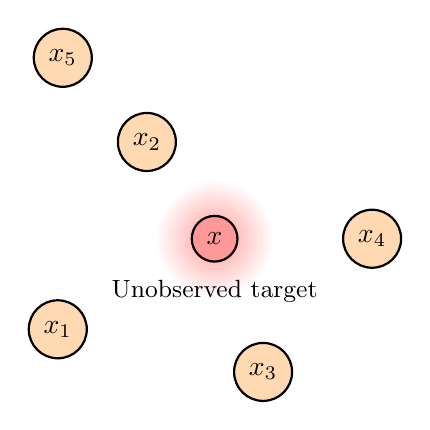
\begin{tikzpicture}

        % Clean target node (not directly used, but for reference)
                \node [shade, inner color=red!40, outer color=white, draw=none, circle, minimum size=1.5cm] (clean_target_halo) {};
        \node [draw, circle, fill=red!40, thick] (clean_target) at (clean_target_halo)  {\textbf{$x$}};
        \node [below=0.1cm] at (clean_target.south) {\small Unobserved target};

        % Multiple noisy targets
        \foreach \i/\angle/\distance in {1/210/2.3, 2/125/1.5, 3/290/1.8, 4/0/2, 5/130/3} {
            \node[draw, circle, fill=orange!30, thick] (noisy\i) at ($(clean_target) + (\angle:\distance)$) {\textbf{$x_{{\i}}$}};
            % \draw[->, thick, opacity=0.4] (pred) -- (noisy\i);
        }
    \end{tikzpicture}
    % \small
    % \textbf{Noise2Noise:} The network learns from multiple noisy targets, each providing a different noisy realization, and the average prediction converges to the clean signal if noise is zero-mean and independent.
\end{frame}

\begin{frame}{Further intuition}{Noise2Noise : restore image without clean data}
    \centering
    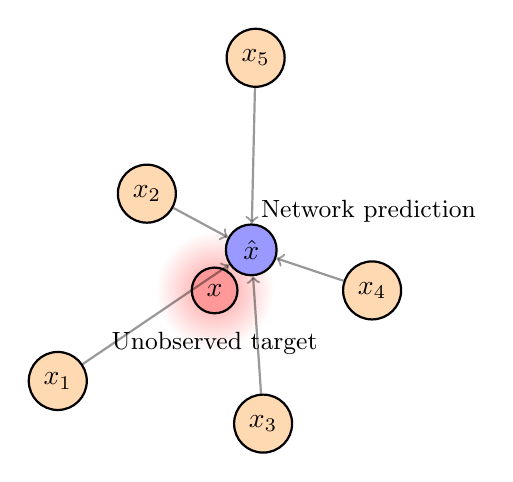
\begin{tikzpicture}

        % Clean target node (not directly used, but for reference)
        \node [shade, inner color=red!40, outer color=white, draw=none, circle, minimum size=1.5cm] (clean_target_halo) {};
        \node [draw, circle, fill=red!40, thick] (clean_target) at (clean_target_halo)  {\textbf{$x$}};
        \node [below=0.1cm] at (clean_target.south) {\small Unobserved target};

        % model prediction node
        \node [draw, circle, fill=blue!40, thick] (pred) at ([xshift=0.25cm, yshift=0.3cm]clean_target.north east) {\textbf{$\hat{x}$}};
        \node [above=0.15cm, anchor=west] at (pred.north) {\small Network prediction};

        % Multiple noisy targets
        \foreach \i/\angle/\distance in {1/210/2.3, 2/125/1.5, 3/290/1.8, 4/0/2, 5/80/3} {
            \node[draw, circle, fill=orange!30, thick] (noisy\i) at ($(clean_target) + (\angle:\distance)$) {\textbf{$x_{{\i}}$}};
            \draw[->, thick, opacity=0.4] (noisy\i) -- (pred);
        }


    \end{tikzpicture}
    % \small
    % \textbf{Noise2Noise:} The network learns from multiple noisy targets, each providing a different noisy realization, and the average prediction converges to the clean signal if noise is zero-mean and independent.
\end{frame}

\section{Positron Emission Tomography (PET) imaging}

\begin{frame}
    \tableofcontents[currentsection, hideallsubsections]
\end{frame}

\begin{frame}{PET introduction}{Positron Emission Tomography (PET) imaging}
    \begin{columns}
        \begin{column}{0.65\textwidth}
            \begin{itemize}
                \item \textbf{PET} is a medical imaging technique that detects pairs of gamma rays emitted by a tracer.
                \item The patient is injected with a radioactive tracer that emits positrons.
                \item When a positron meets an electron, they annihilate, producing two gamma photons detected by a ring of detectors.
                \item The data collected is used to reconstruct images of tracer concentration in the body.
            \end{itemize}
        \end{column}
        \begin{column}{0.35\textwidth}
            \centering
            % PET principle illustration (already present)
             \begin{figure}
                    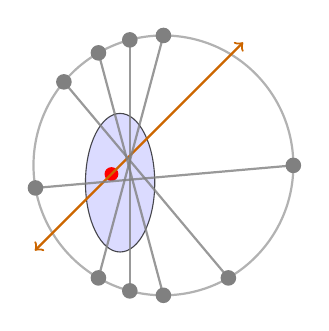
\begin{tikzpicture}[scale=1.1]
                        % PET scanner ring
                        \draw[thick, gray!60] (0,0) circle (1.5);
                        % Patient ellipse
                        \draw[fill=blue!20, opacity=0.7] (-0.5,-0.2) ellipse (0.4 and 0.8);
                        % Emission point
                        \fill[red] (-0.6,-0.1) circle (0.08);
                        % Gamma rays from emission point (aligned, opposite directions)
                        \draw[->, thick, orange!80!black] (-0.6,-0.1) -- ++(45:2.15);
                        \draw[->, thick, orange!80!black] (-0.6,-0.1) -- ++(225:1.25);
                        % Coincident green points at irregular locations
                        \foreach \i/\a/\b in {
                              1/0/190,
                              2/90/240,
                              3/105/255,
                              4/120/270,
                              5/140/300
                        } {
                            % Place green points on the ring
                            \fill[black!50] ({1.5*cos(\a)}, {1.5*sin(\a)}) circle (0.09);
                            \fill[black!50] ({1.5*cos(\b)}, {1.5*sin(\b)}) circle (0.09);
                            % Draw coincident line (not perfectly intersecting)
                            \draw[thick, black!50, opacity=0.8] ({1.5*cos(\a)}, {1.5*sin(\a)}) -- ({1.5*cos(\b)}, {1.5*sin(\b)});
                        }
                    \end{tikzpicture}
            \caption{PET : Emission event detected by ring detectors}
            \end{figure}

        \end{column}
    \end{columns}
\end{frame}


\begin{frame}{PET reconstruction as a linear inverse problem}{Positron Emission Tomography (PET) imaging}
    \begin{center} $\vcenter{\hbox{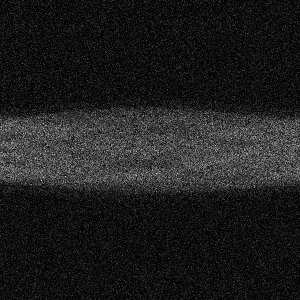
\includegraphics[scale=0.25]{simu_pt.jpg}}}
= \text{Poisson}\left( A \cdot
\vcenter{\hbox{
\includegraphics[scale=0.5, trim = 20 20 20 20, clip]{gt_web_after_scaling.png}}} + b
\right) $\end{center}
\vspace{0.5cm}
    \begin{itemize}
        \item The PET reconstruction problem can be formulated as a Poisson linear inverse problem :
        \begin{equation}
            Y | X=x\sim \text{Poisson}(Ax + b)
        \end{equation}
        \item $A$ is \textbf{known} and is the \textbf{system/projection matrix}.
        \item $b$ is task-specific error term (scatter, randoms) and can be estimated.
    \end{itemize}
{\color{lightgray}\scriptsize Image source : BrainWeb, \url{https://brainweb.bic.mni.mcgill.ca/brainweb/}}
\end{frame}

\begin{frame}{PET matrix system}{Positron Emission Tomography (PET) imaging}
    \begin{equation}
        A = P_\text{detector} \cdot N \cdot R \cdot P_\text{image}
    \end{equation}
    \begin{itemize}
        \item $P_\text{detector}$ : Sinogram PSF (blurring effect after projection modeling resolution effects)
        \item $N$ : Attenuation matrix (photon absorption in tissue)
        \item $R$ : geometric projection matrix (e.g. Radon transform)
        \item $P_\text{image}$ : Image PSF (blurring effect before projection)
    \end{itemize}
\end{frame}

\begin{frame}{PET reconstruction methods}{Positron Emission Tomography (PET) imaging}
    \begin{figure}
        \begin{tikzpicture}
            % placer l'image dans un nœud
            \node (sino) {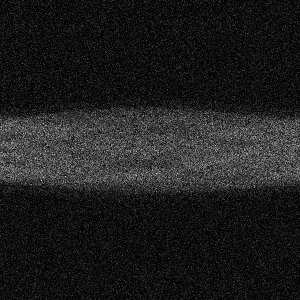
\includegraphics[scale=0.27]{simu_pt.jpg}};
            \node (sino_label) [below=of sino, yshift=0.5cm] {Sinogramm};

            \node (brain_fbp) [right=of sino, xshift=1cm, yshift=1.5cm] {\includegraphics[scale=0.25, trim = 35 35 35 35, clip]{prompt_fbp.png}};
            \node (brain_mlem) [right=of sino, xshift=1cm, yshift=-1.5cm] {\includegraphics[scale=0.25, trim = 35 35 35 35, clip]{prompt_mlem.png}};

            \draw[->, thick] (sino) -- (brain_fbp) node[midway, fill=white] {FBP};
            \draw[->, thick] (sino) -- (brain_mlem) node[midway, fill=white] {MLEM};
        \end{tikzpicture}
    \caption{PET reconstruction examples from simulated data.}
    \end{figure}
{\color{lightgray}\scriptsize Image source : author}
\end{frame}

\begin{frame}{PET : ground truth unavailability}{Positron Emission Tomography (PET) imaging}

    \begin{figure}
        \begin{columns}
            \begin{column}{0.3\textwidth}
                \centering
                \begin{adjustbox}{max totalsize={\textwidth}{0.8\textheight}}
                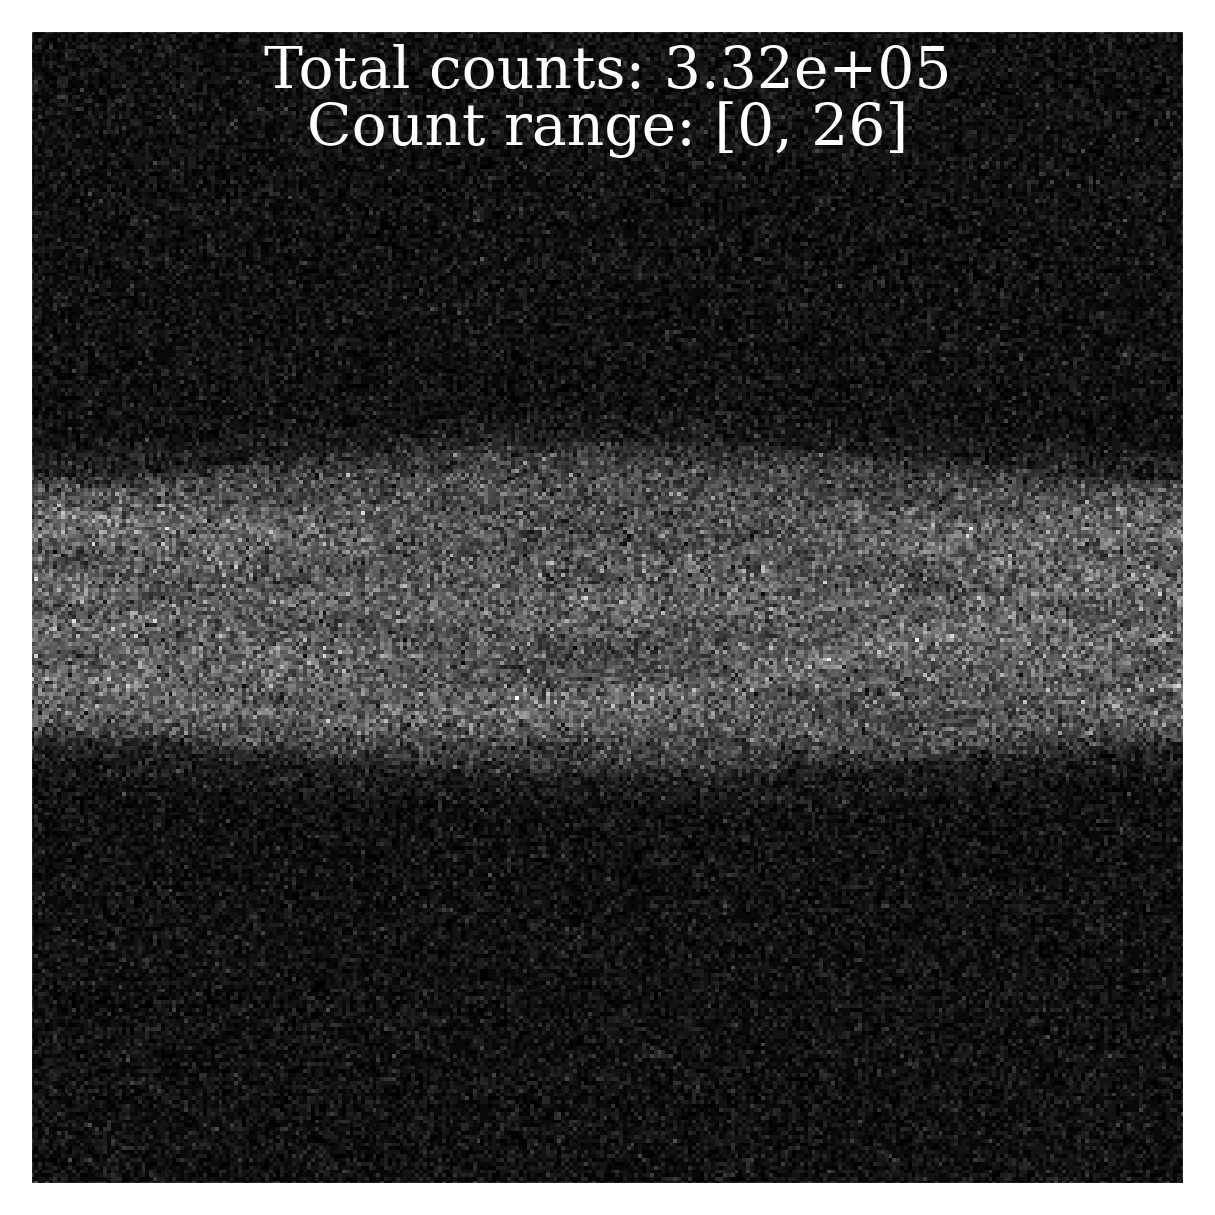
\includegraphics{prompt_03M.png}
                \end{adjustbox}
            \end{column}
            \begin{column}{0.3\textwidth}
                \centering
                \begin{adjustbox}{max totalsize={\textwidth}{0.8\textheight}}
                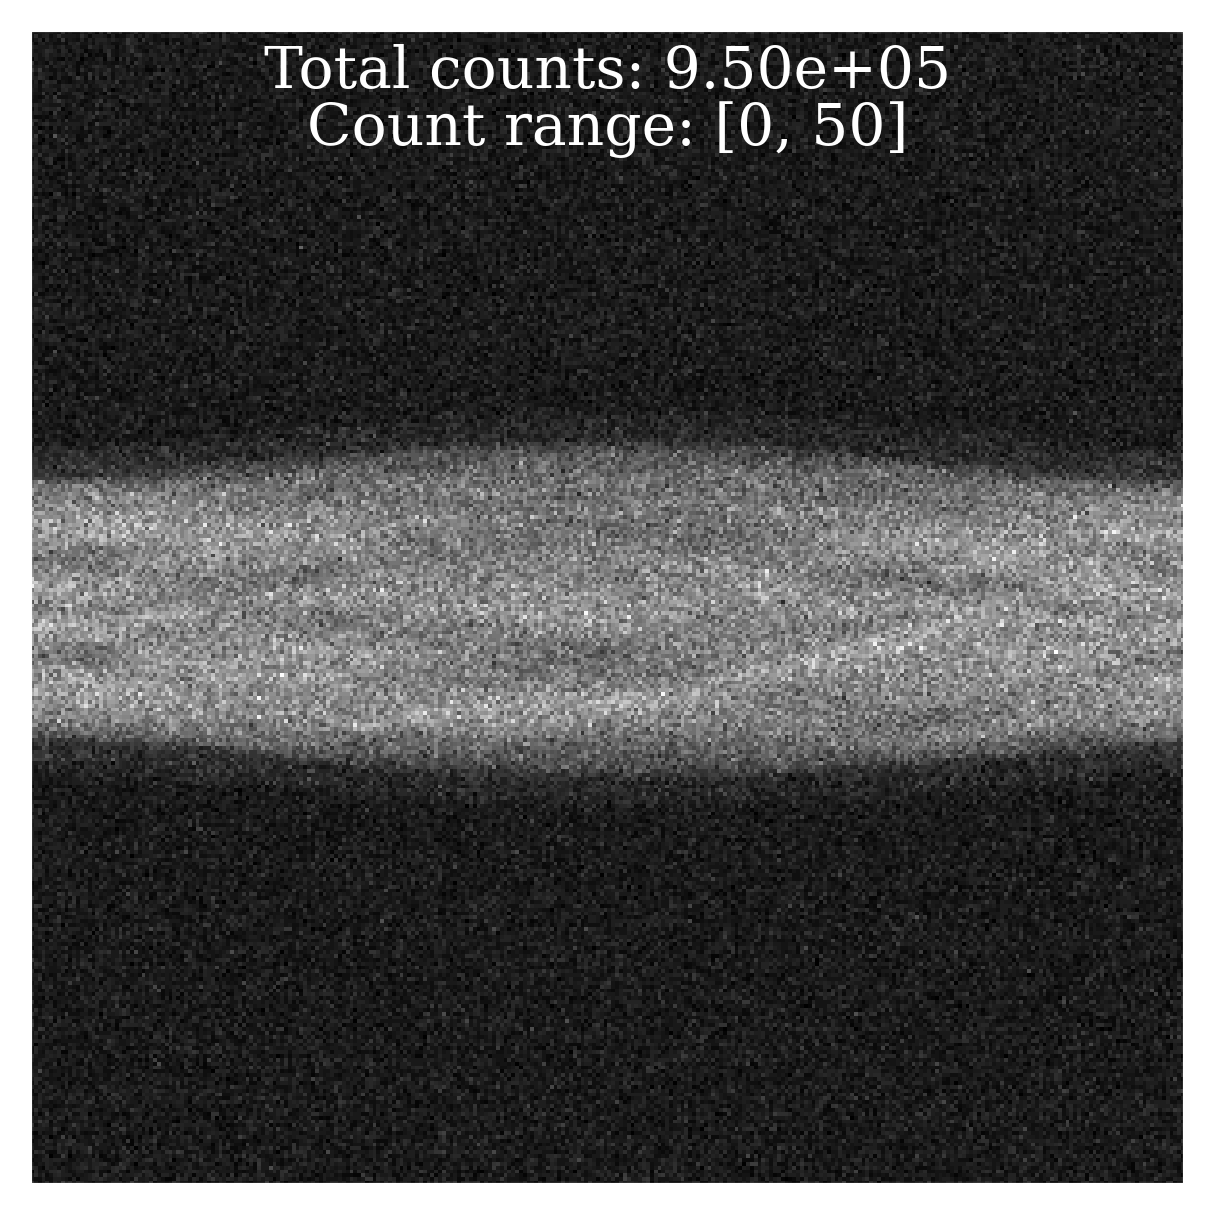
\includegraphics{prompt_1M.png}
                \end{adjustbox}
            \end{column}
            \begin{column}{0.3\textwidth}
                \centering
                \begin{adjustbox}{max totalsize={\textwidth}{0.8\textheight}}
                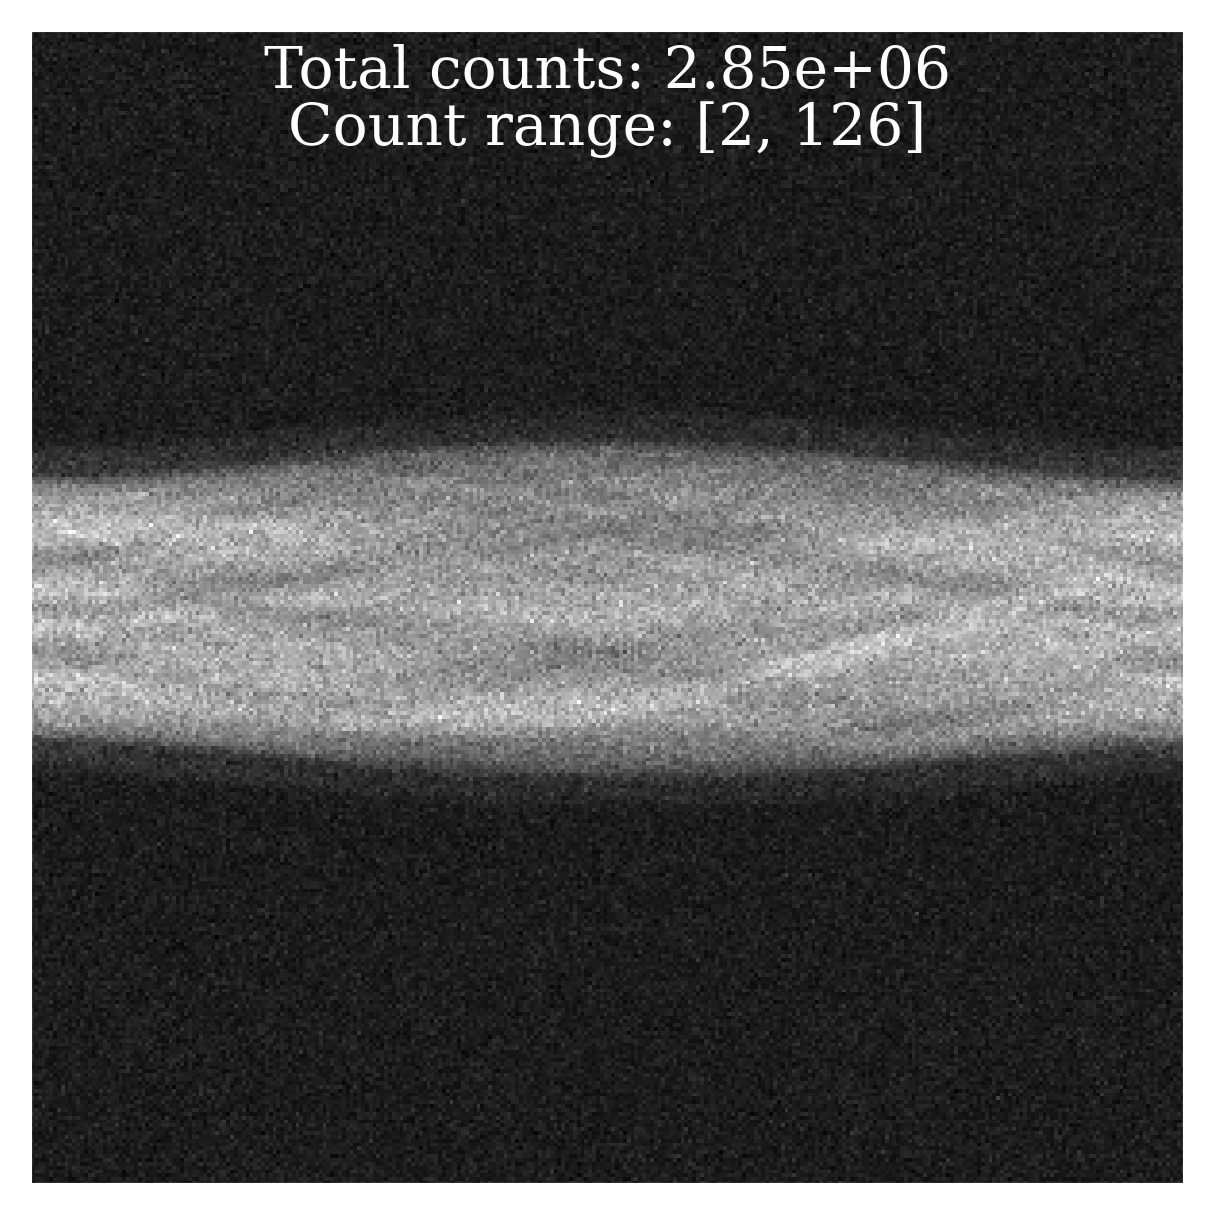
\includegraphics{prompt_3M.png}
                \end{adjustbox}
            \end{column}
        \end{columns}
    \caption{PET : Noisy prompt sinograms with different count levels}
    \end{figure}

    \begin{itemize}
        \item Raw data is noisy and reference high-count sinograms (right) are less available.
        \item Ground truth images are not available at all.
    \end{itemize}
    
\end{frame}

\section{Noise2Noise for PET reconstruction/denoising}

\begin{frame}
    \tableofcontents[currentsection, hideallsubsections]
\end{frame}

\begin{frame}{Binomial sampling}{Noise2Noise for PET reconstruction/denoising}

    \begin{proposition}
        $Y|X$ is $2$-divisible.

        For instance, $Y_i | X=x \sim \text{Binomial}(Ax, \frac{1}{2})$ works and :
        \begin{equation}
            \begin{cases}
                Y_i | X \sim \text{Poisson}(\frac{1}{2}Ax) \\
                Y_1 | X \perp\!\!\!\!\perp Y_2 | X.
            \end{cases}  
        \end{equation}

        Hence, statistical conditions \ref{statistical-conditions} are satisfied and Noise2Noise can be applied.
         \label{n2n-prop-divisible}
    \end{proposition}

    This a special case of "GeneralizedRecorrupted2Recorrupted" \cite{gr2r}.
\end{frame}

\begin{frame}{Binomial sampling}{Noise2Noise for PET reconstruction/denoising}
    \centering
    \begin{figure}
        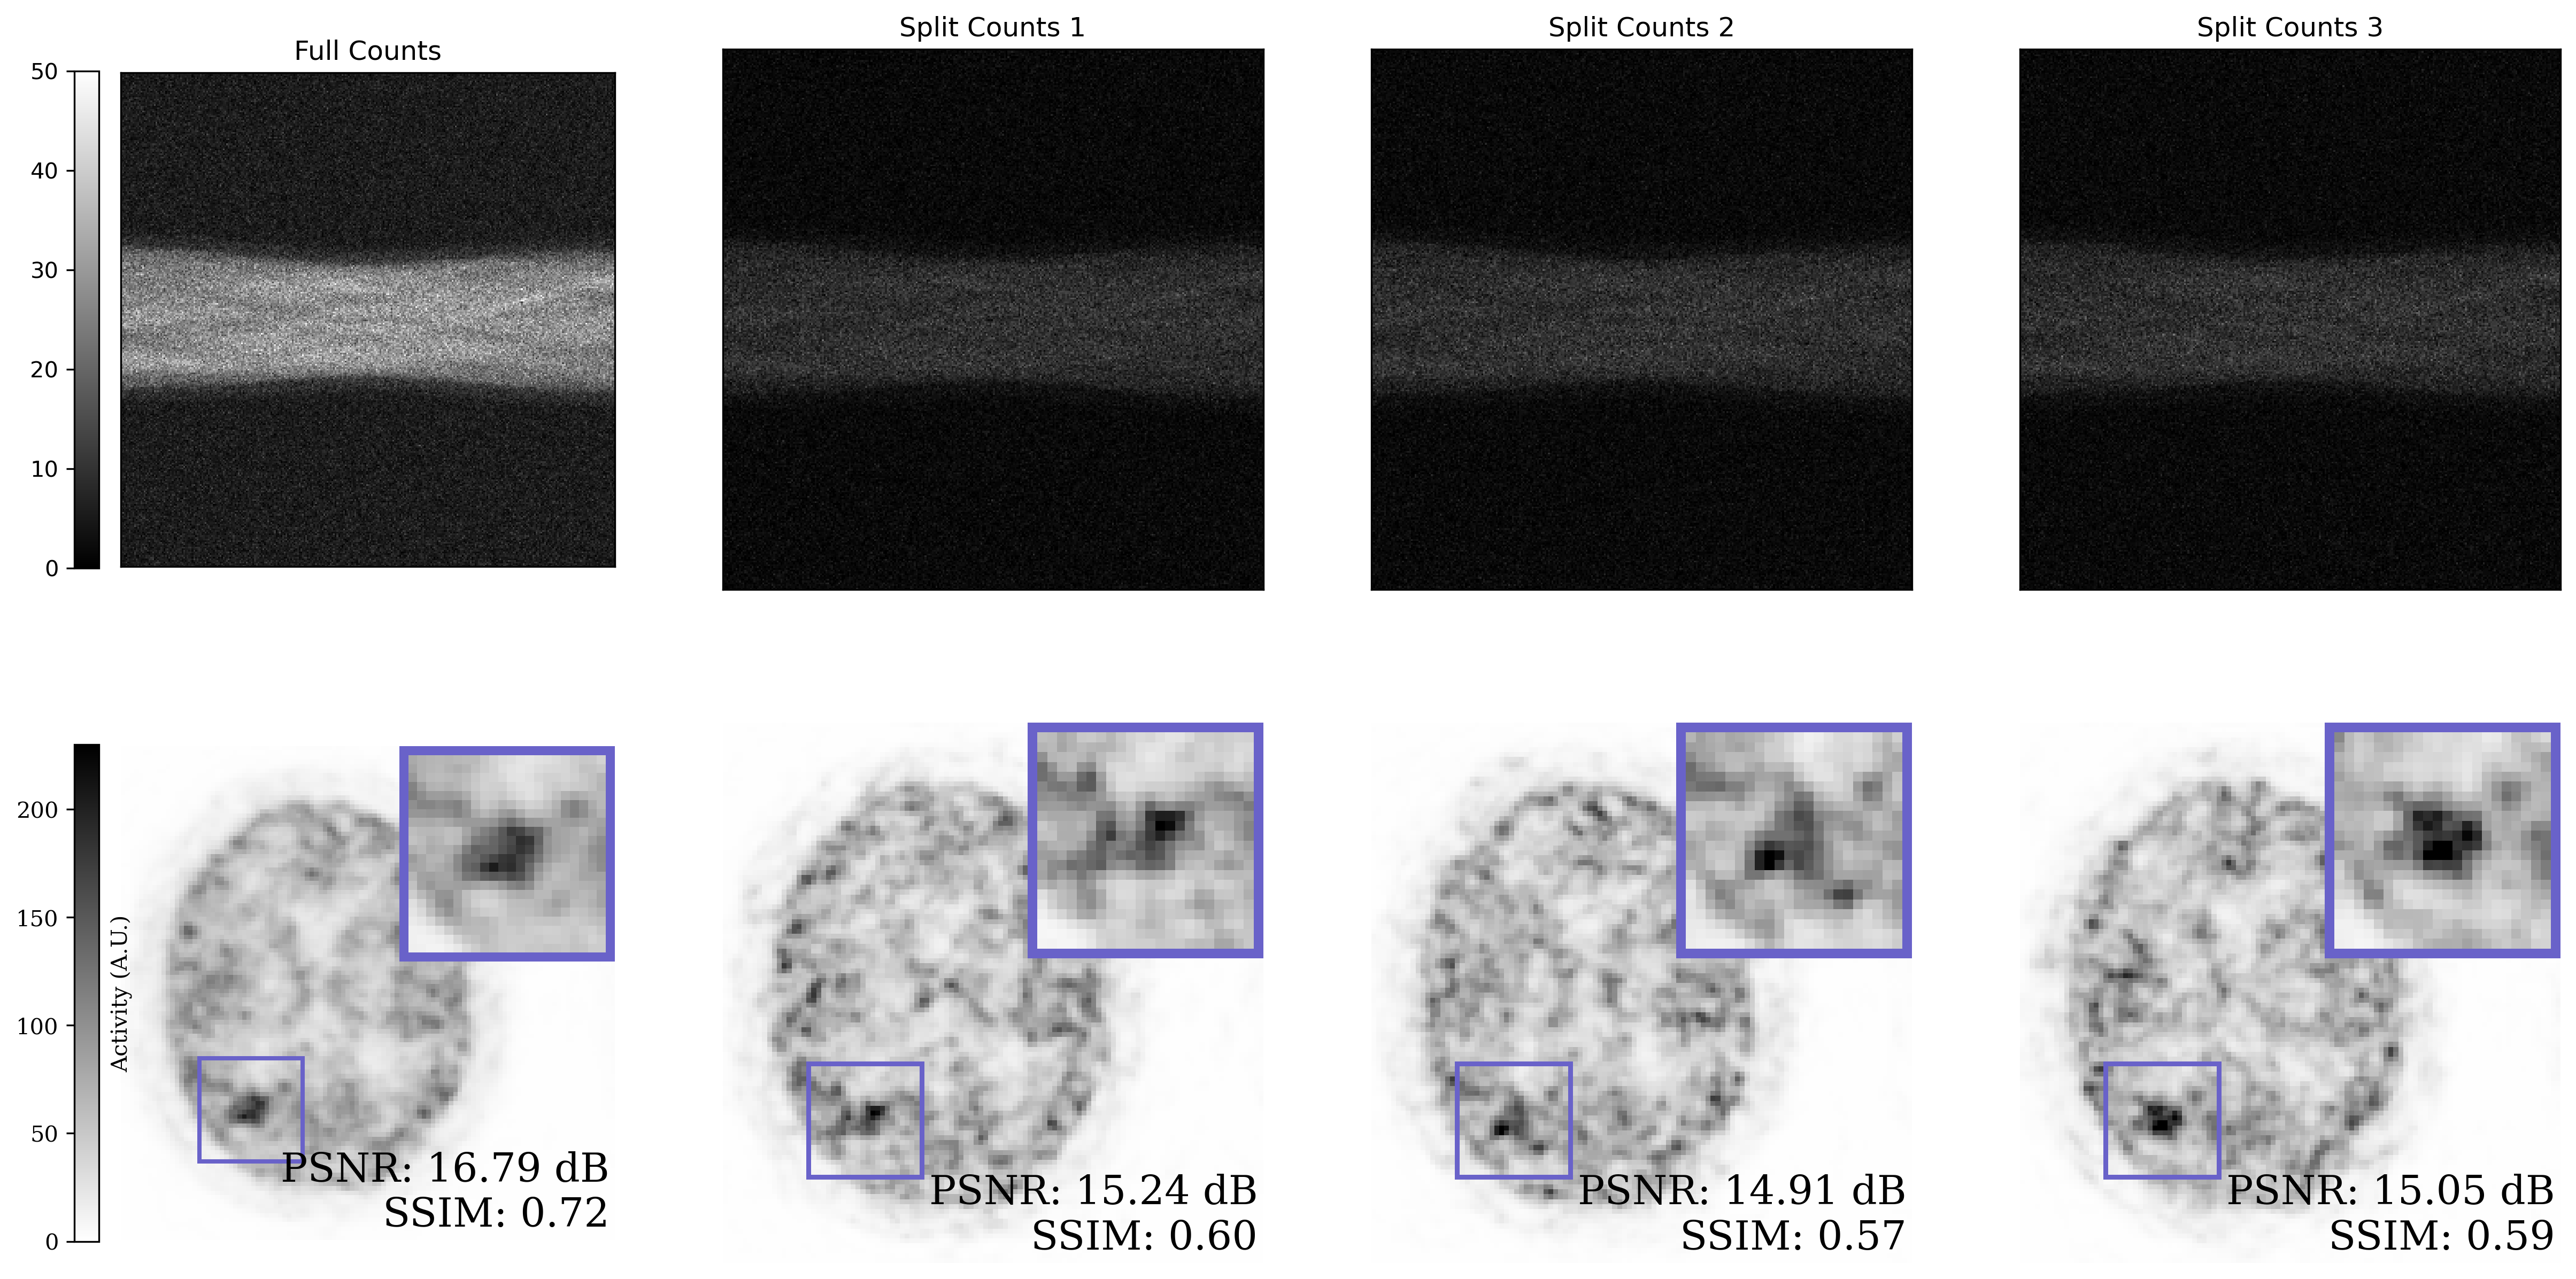
\includegraphics[scale=0.07]{split.png}
        \caption{Sinogram binomial splitting $Y_i | X=x \sim \text{Binomial}(Ax, \frac{1}{3})$ and their corresponding reconstructions.}
    \end{figure}
\end{frame}

\begin{frame}{Implementation details}{Noise2Noise for PET reconstruction/denoising}
    \begin{figure}
        \centering
        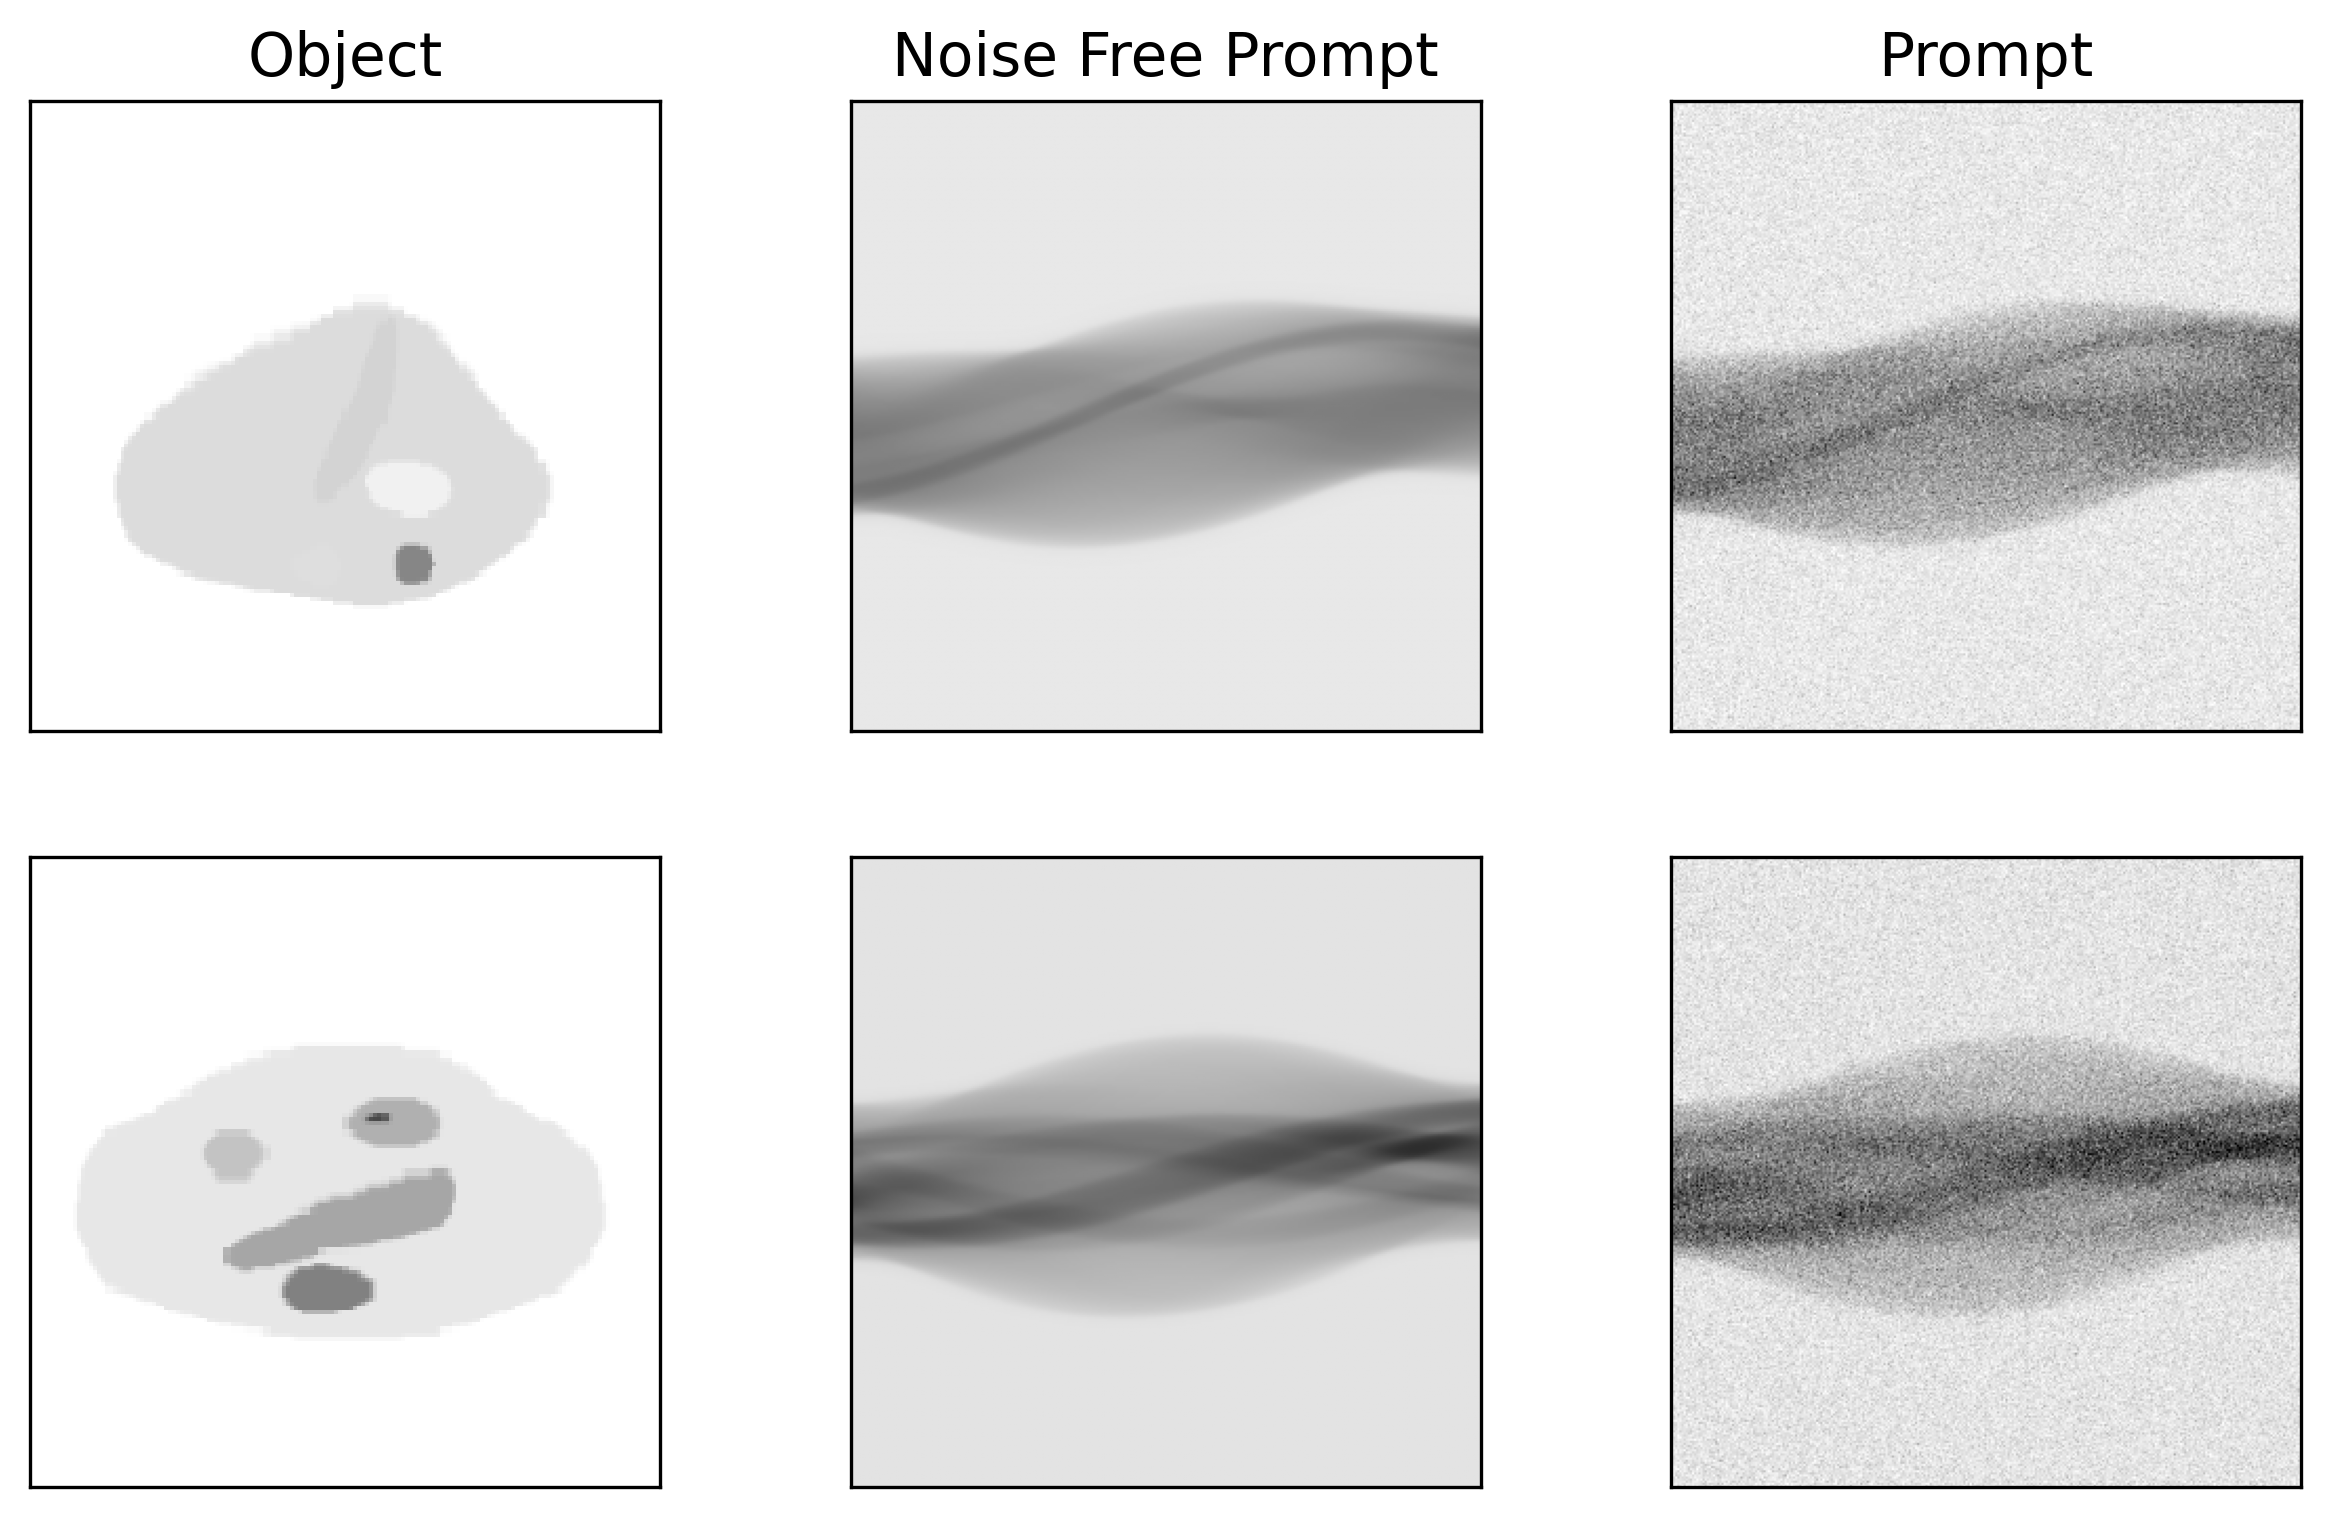
\includegraphics[scale=.125]{phantom.png}
        \caption{Synthetic distribution map and their corresponding sinograms.}
    \end{figure}
{\color{lightgray}\scriptsize Image source : author}
\end{frame}

\begin{frame}{Methodology}{Noise2Noise for PET reconstruction/denoising}
    \centering
    \begin{figure}
        \begin{tikzpicture}
            \tiny
            \node (full_sino) {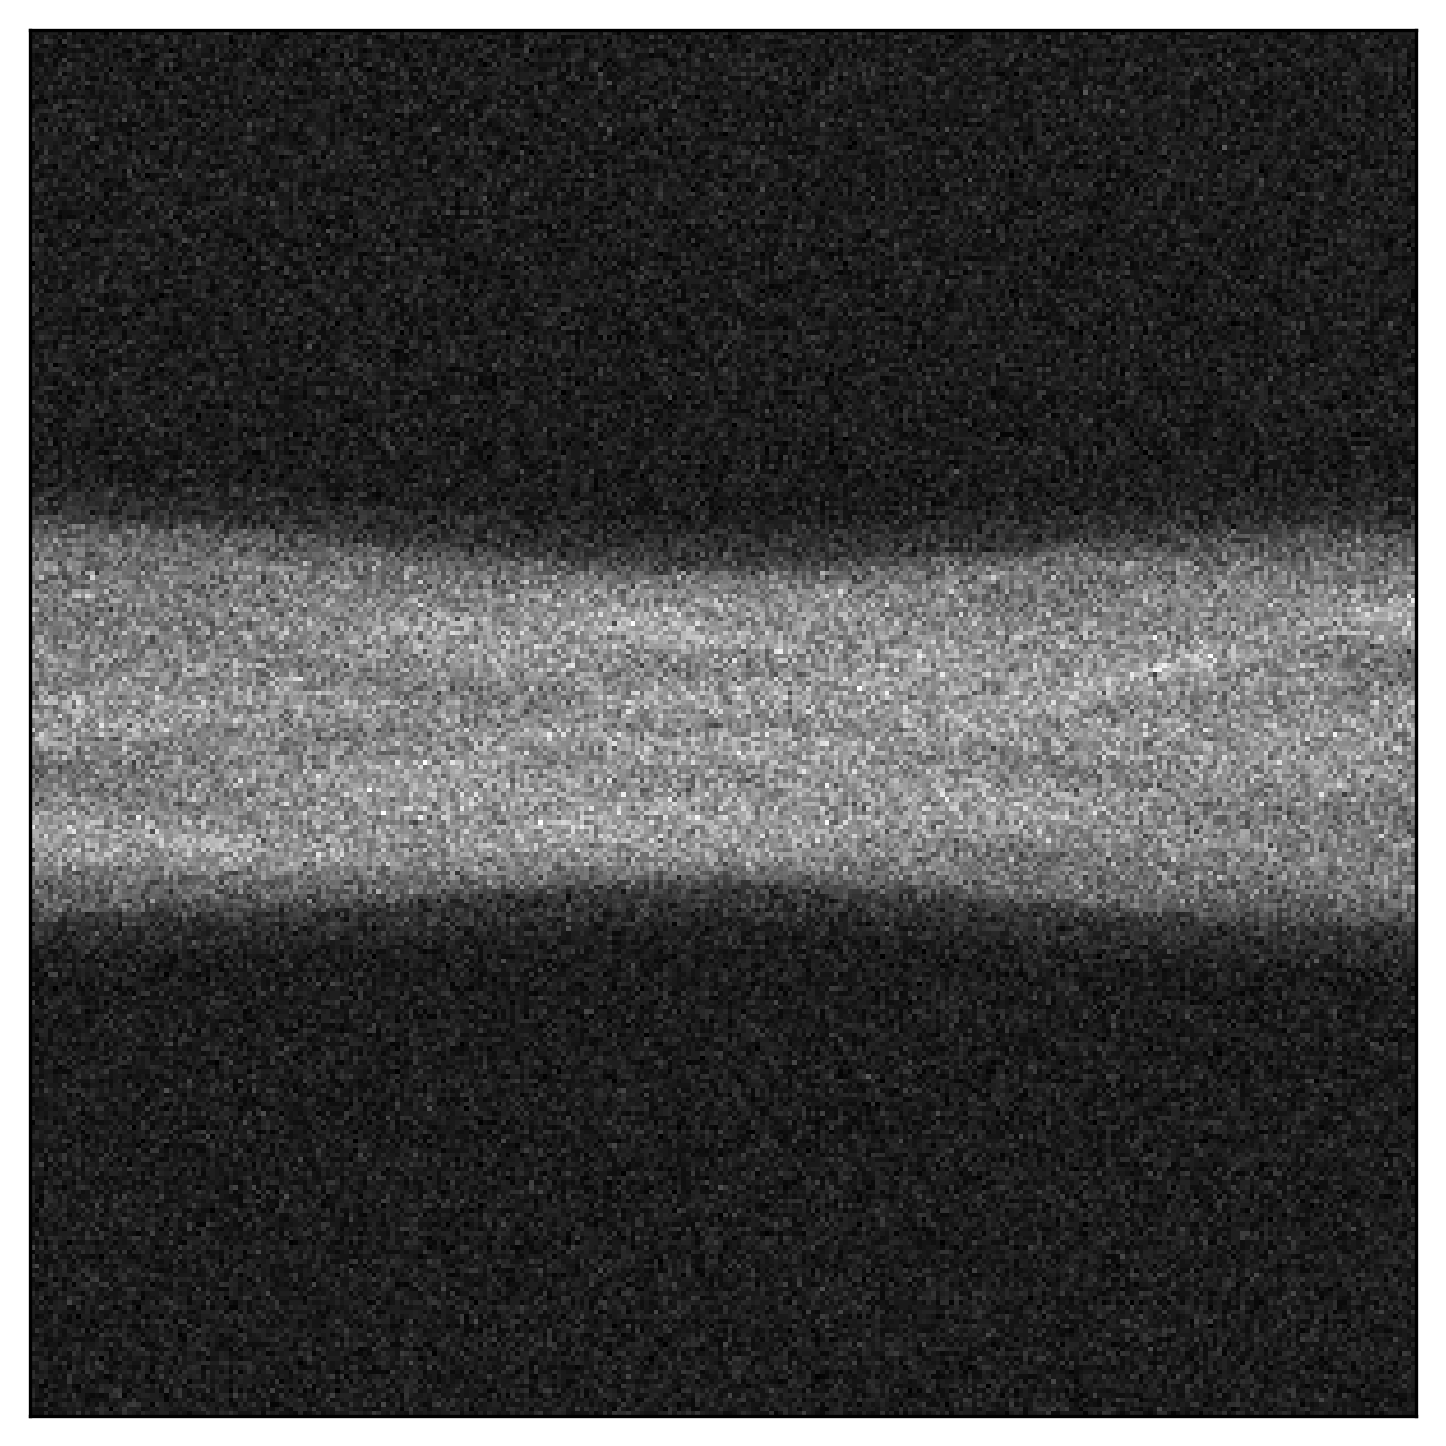
\includegraphics[scale=0.15]{image_to_image/prompt.png}};
            \node [right=0.1cm of full_sino] {Sampling};
            \node (bin0) [right=0.45cm of full_sino, yshift=-1.5cm] {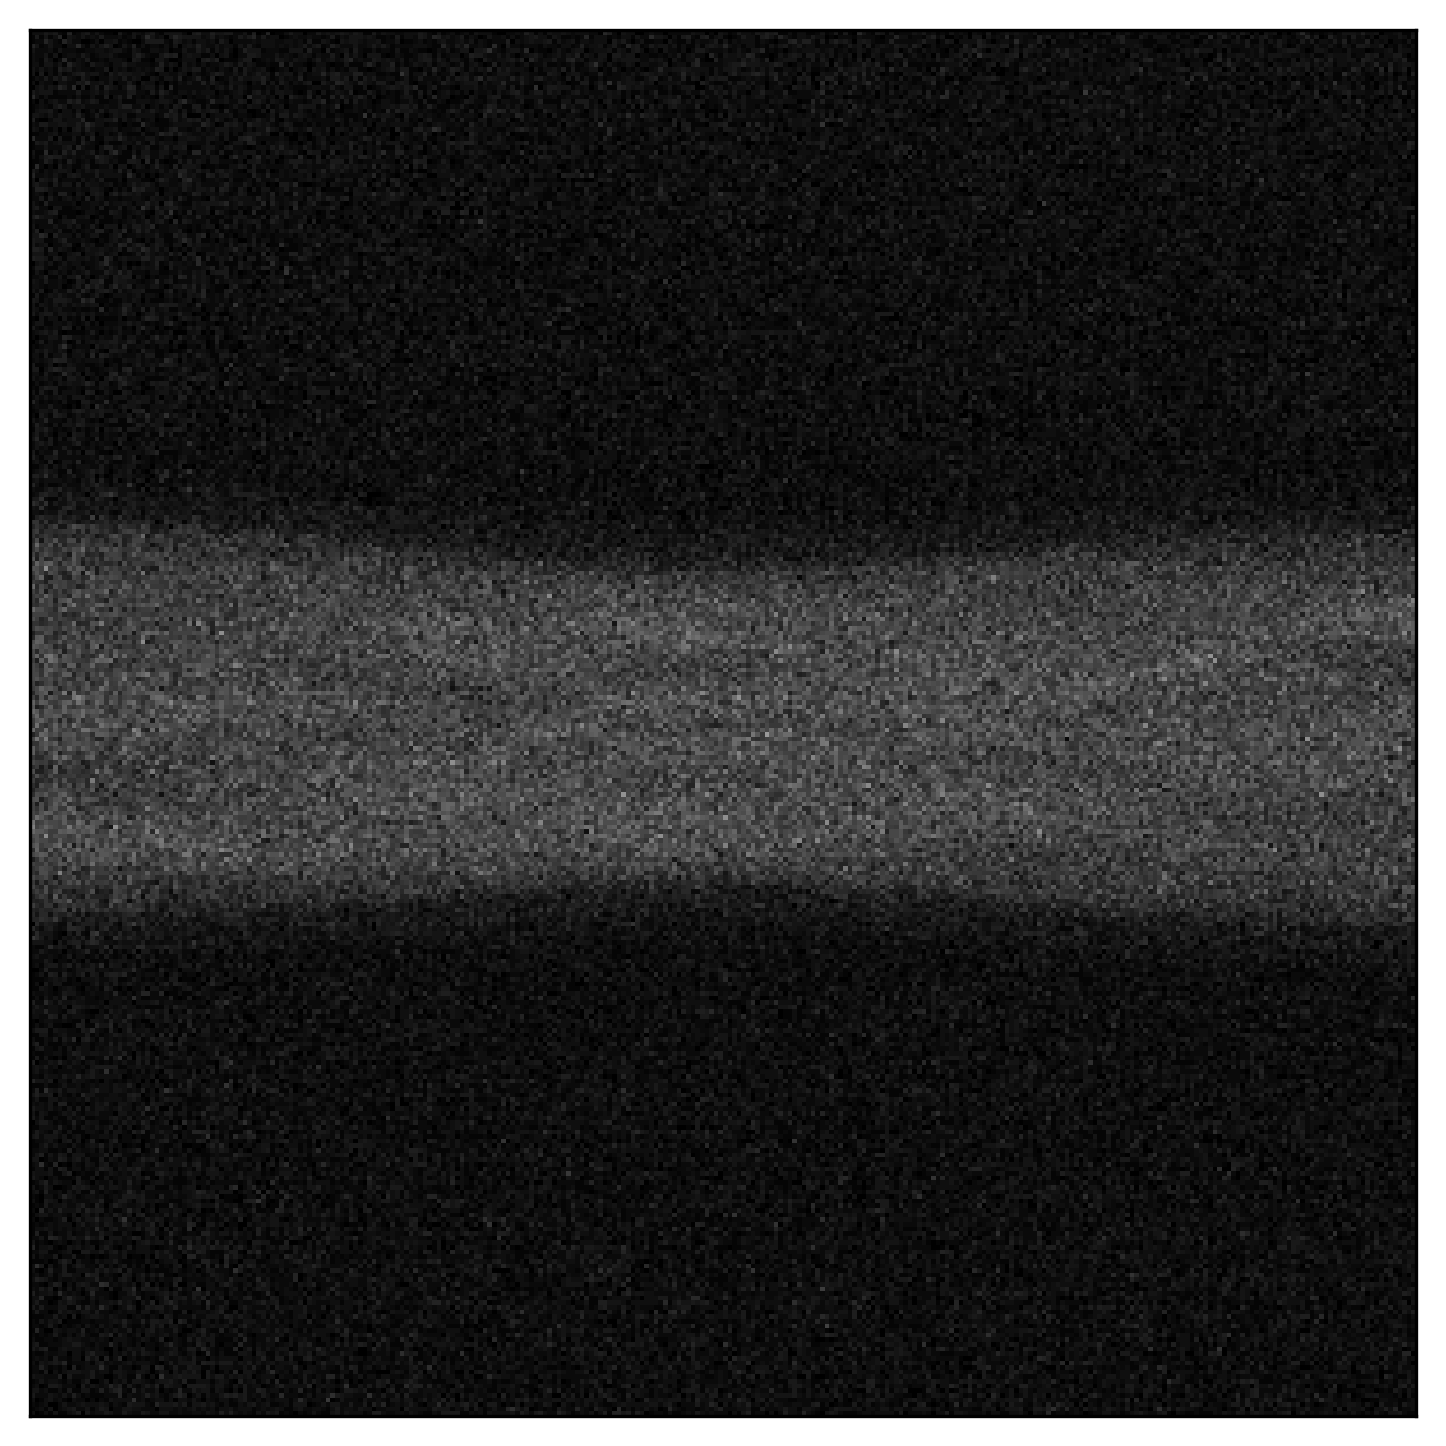
\includegraphics[scale=0.15]{image_to_image/prompt1.png}};
            \node (bin1) [right=0.45cm of full_sino, yshift=1.5cm] {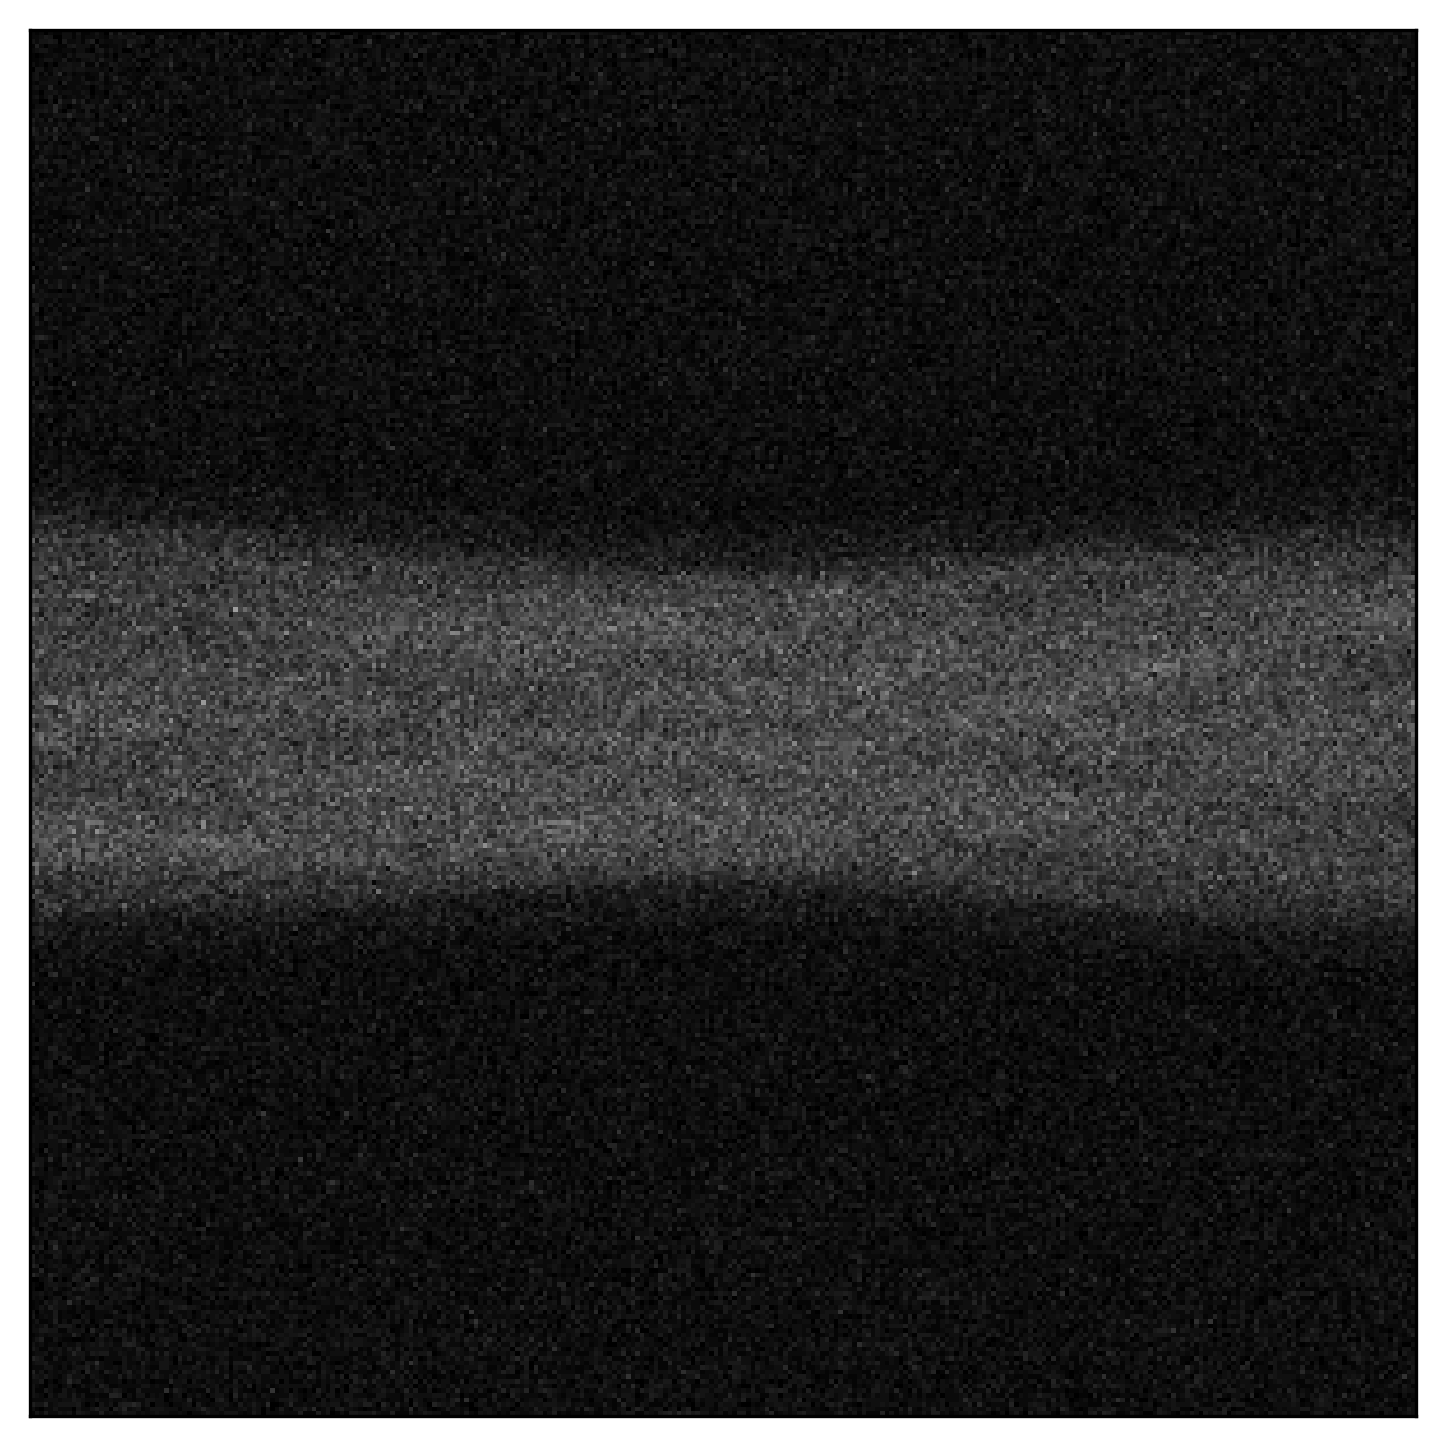
\includegraphics[scale=0.15]{image_to_image/prompt2.png}};

            \node (brain_0) [right=0.45cm of bin0] {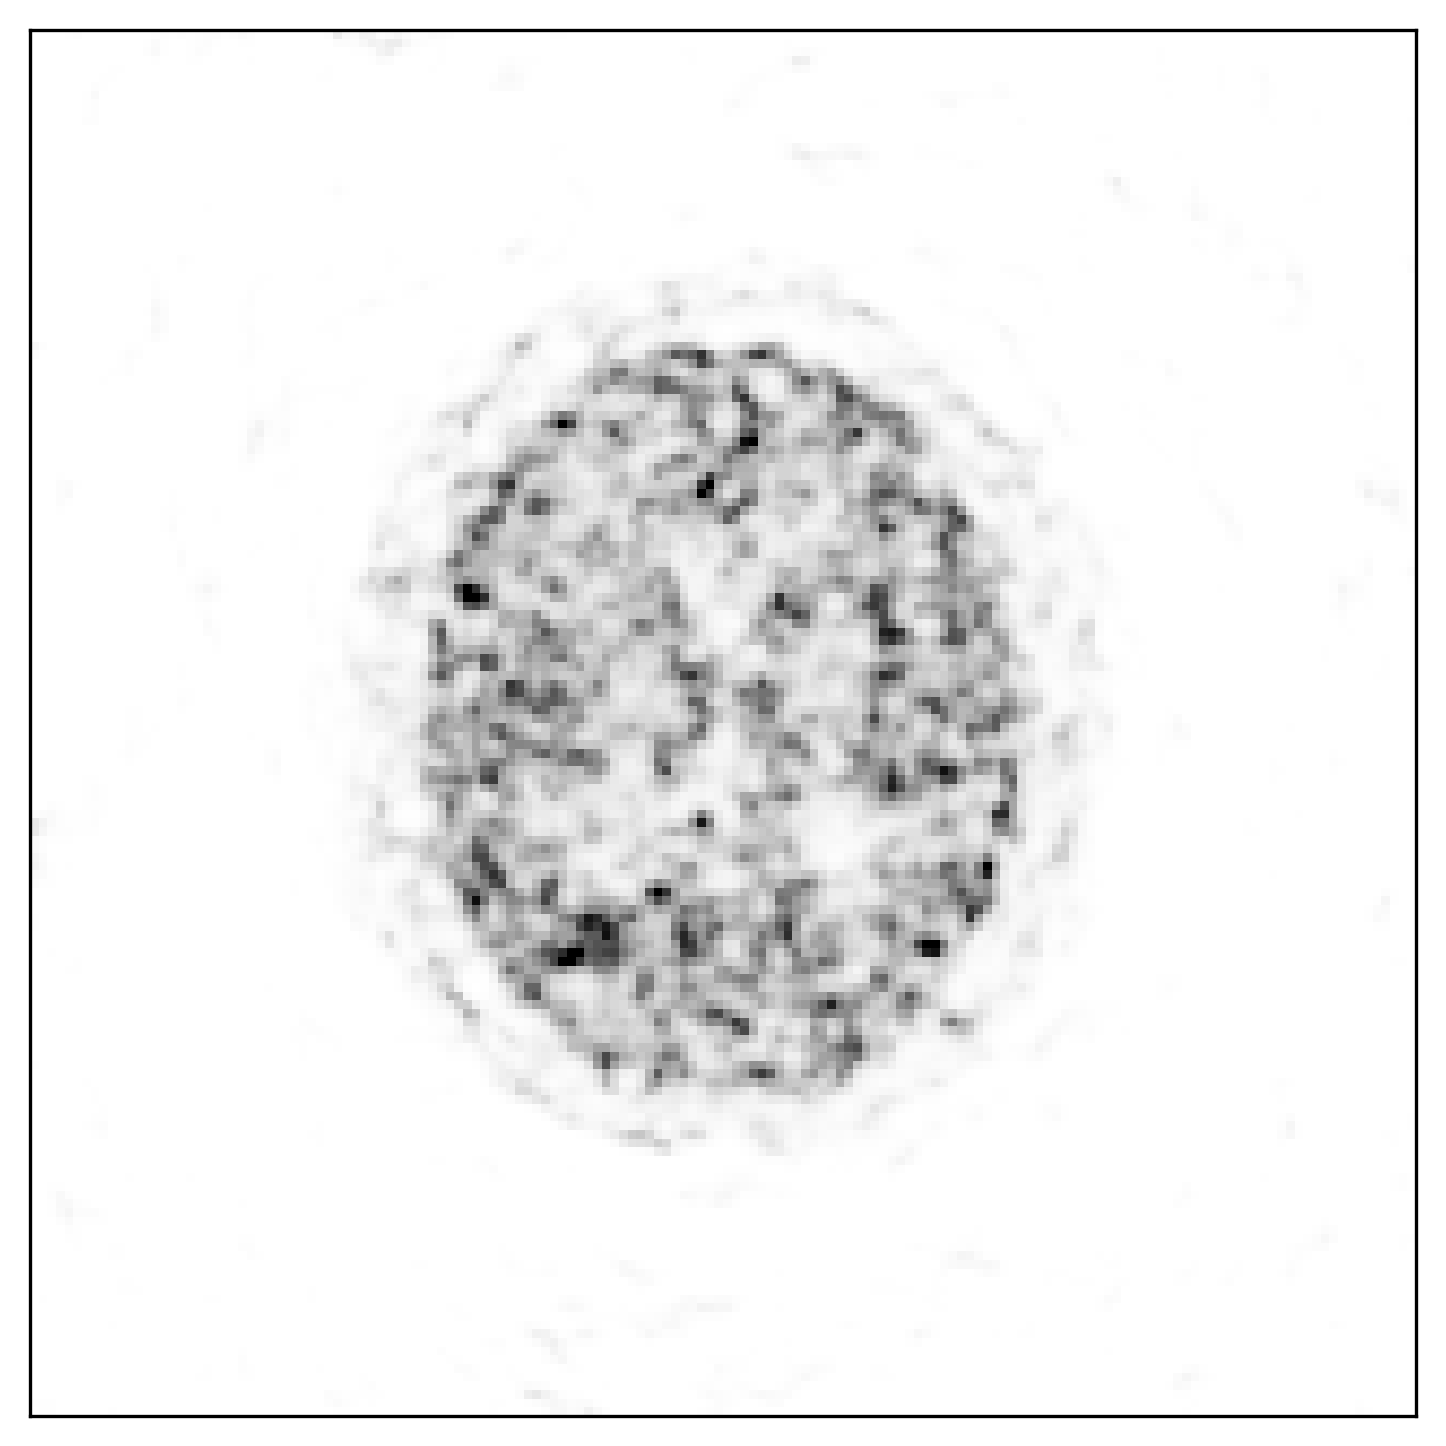
\includegraphics[scale=0.15]{image_to_image/mlem1.png}};
            \node (brain_1) [right=0.45cm of bin1] {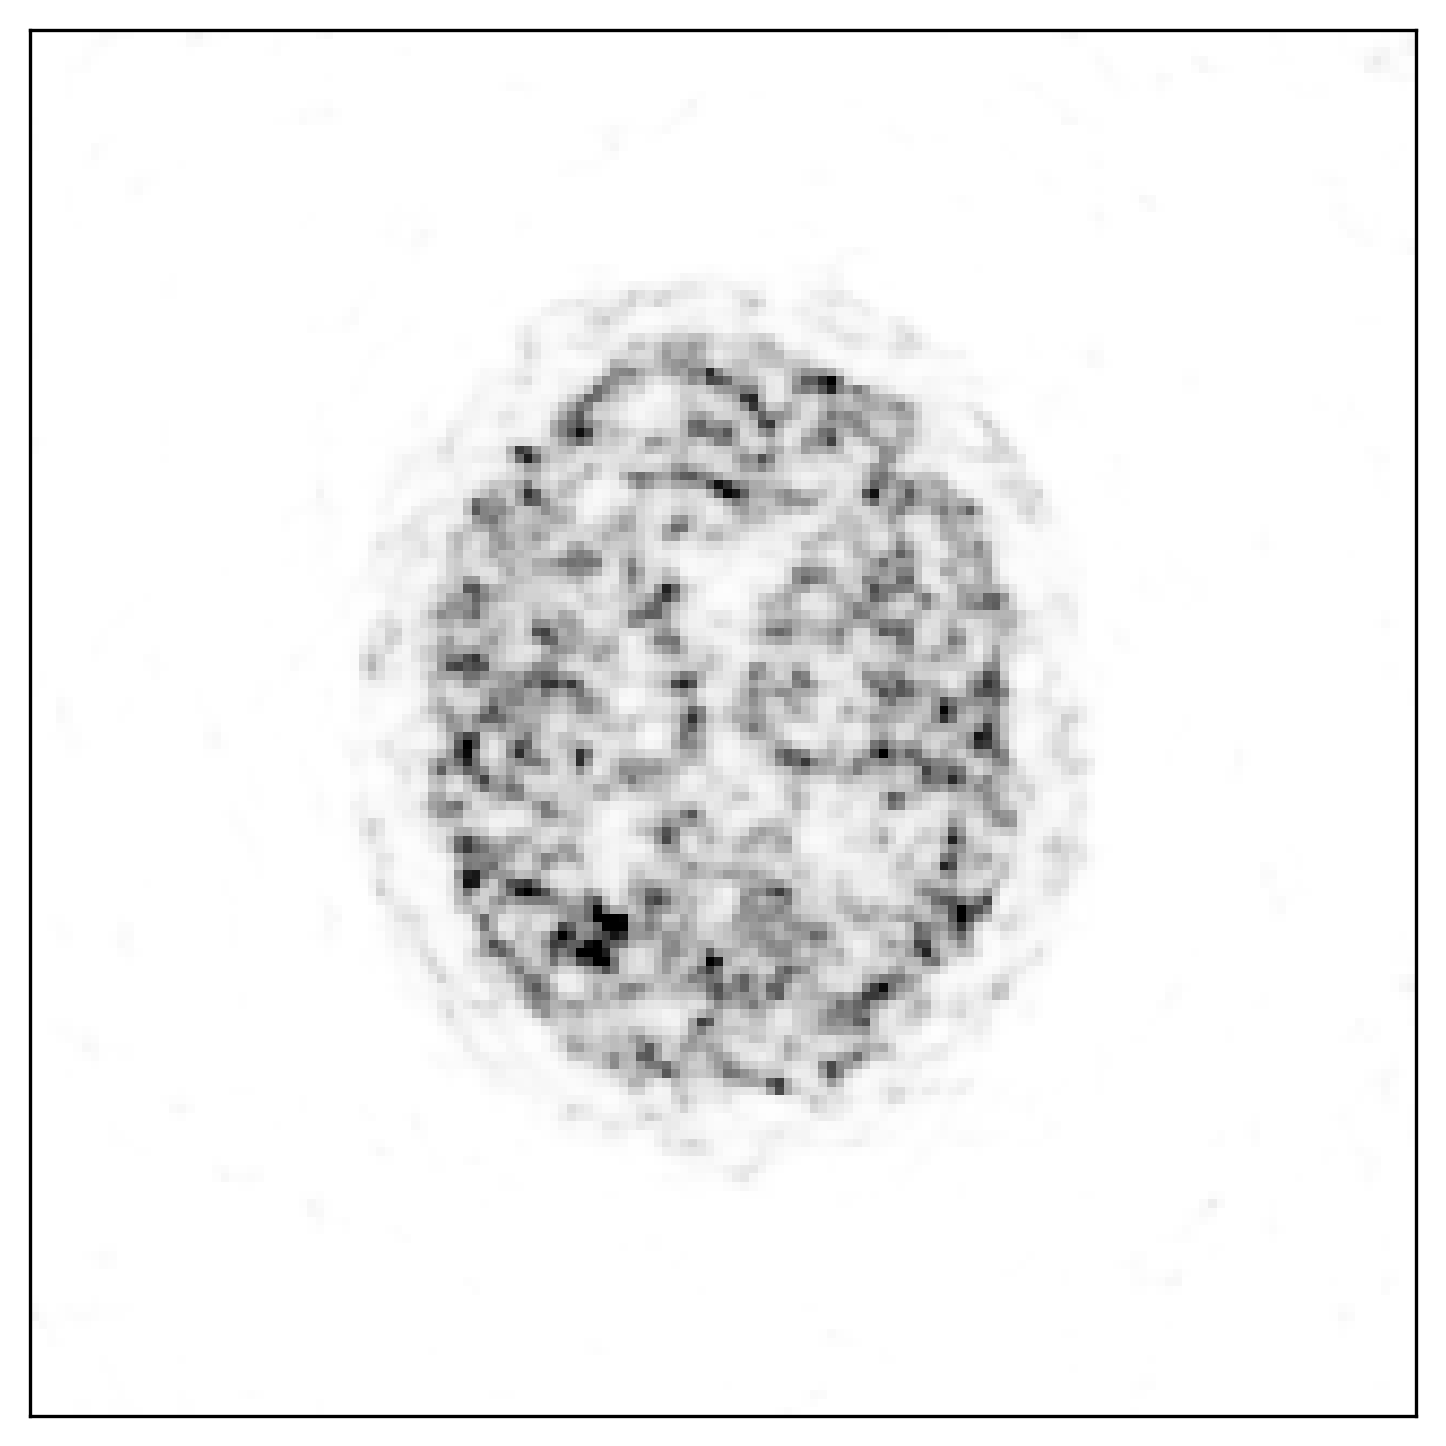
\includegraphics[scale=0.15]{image_to_image/mlem2.png}};

            \node (recon_bin_0) [right=0.45cm of brain_0] {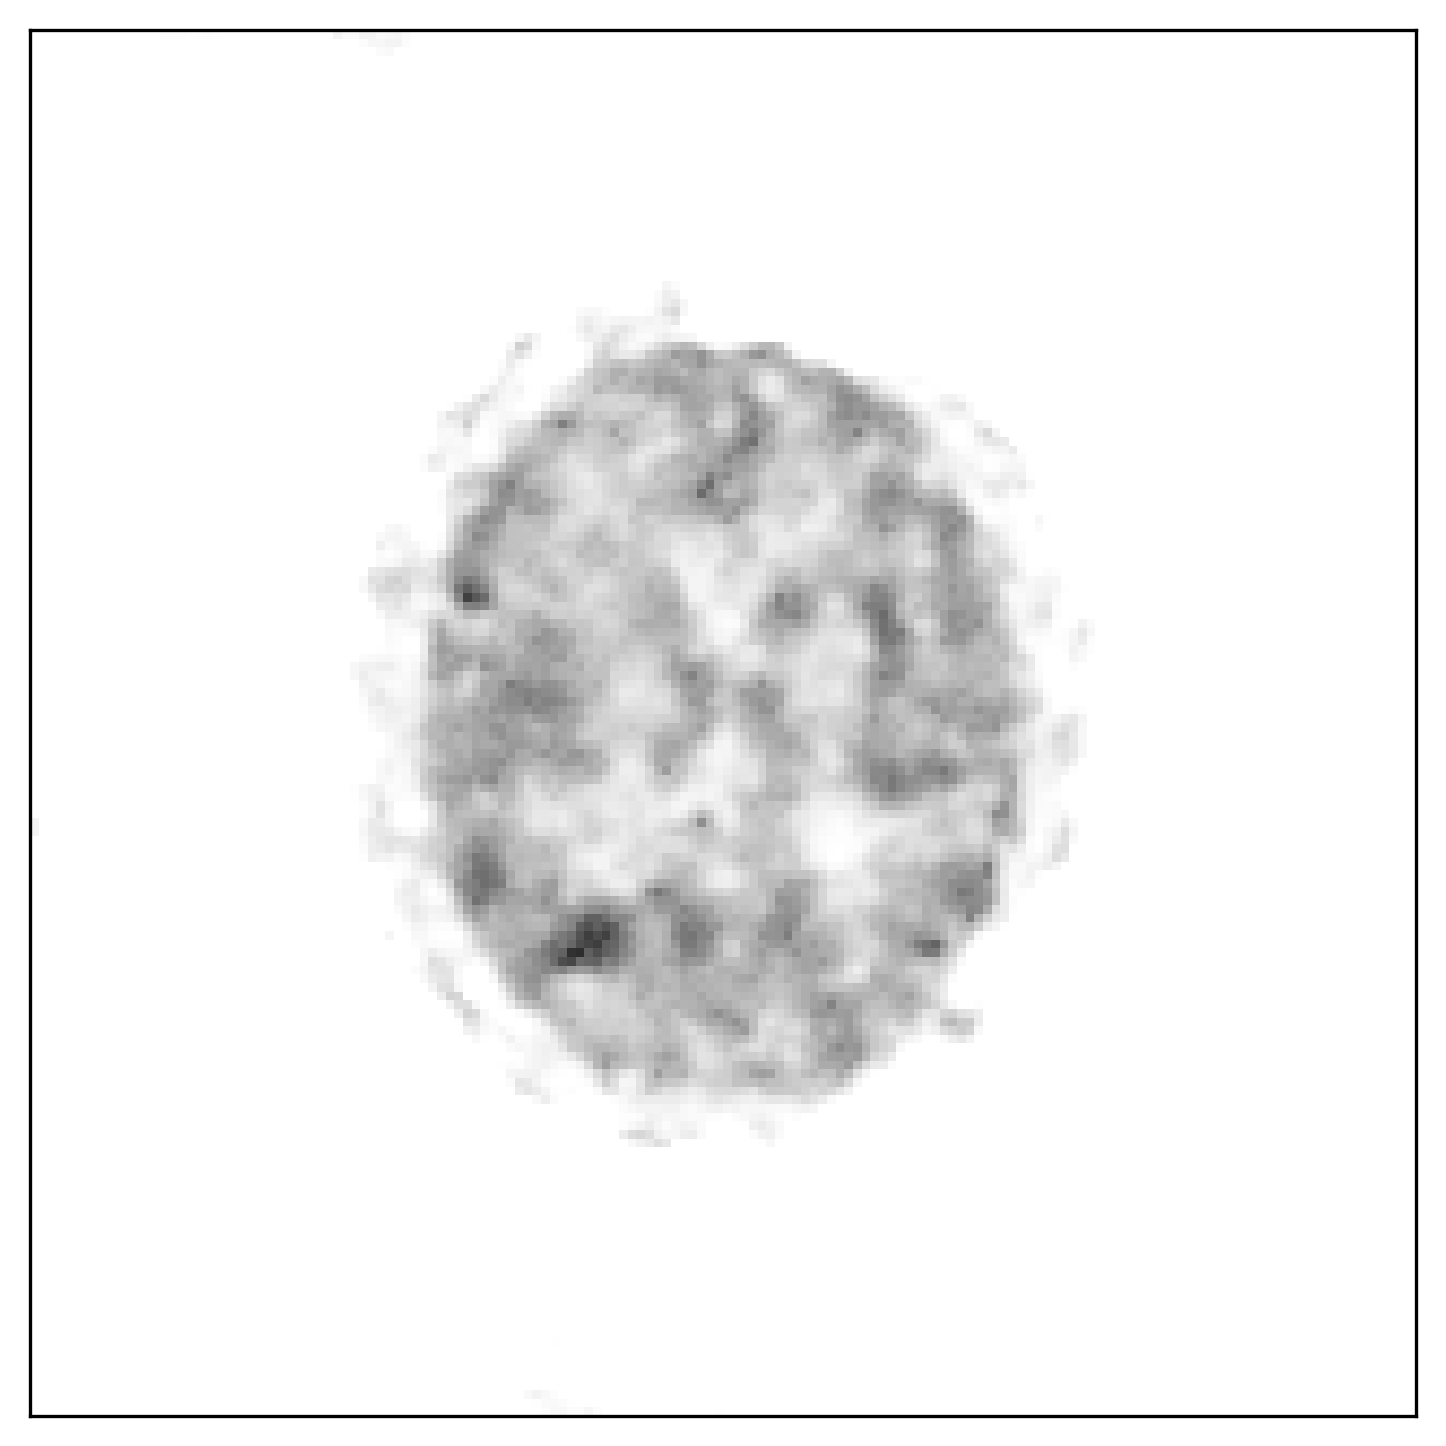
\includegraphics[scale=0.15]{image_to_image/mlem1_denoised.png}};
            \node (recon_bin_1) [right=0.45cm of brain_1] {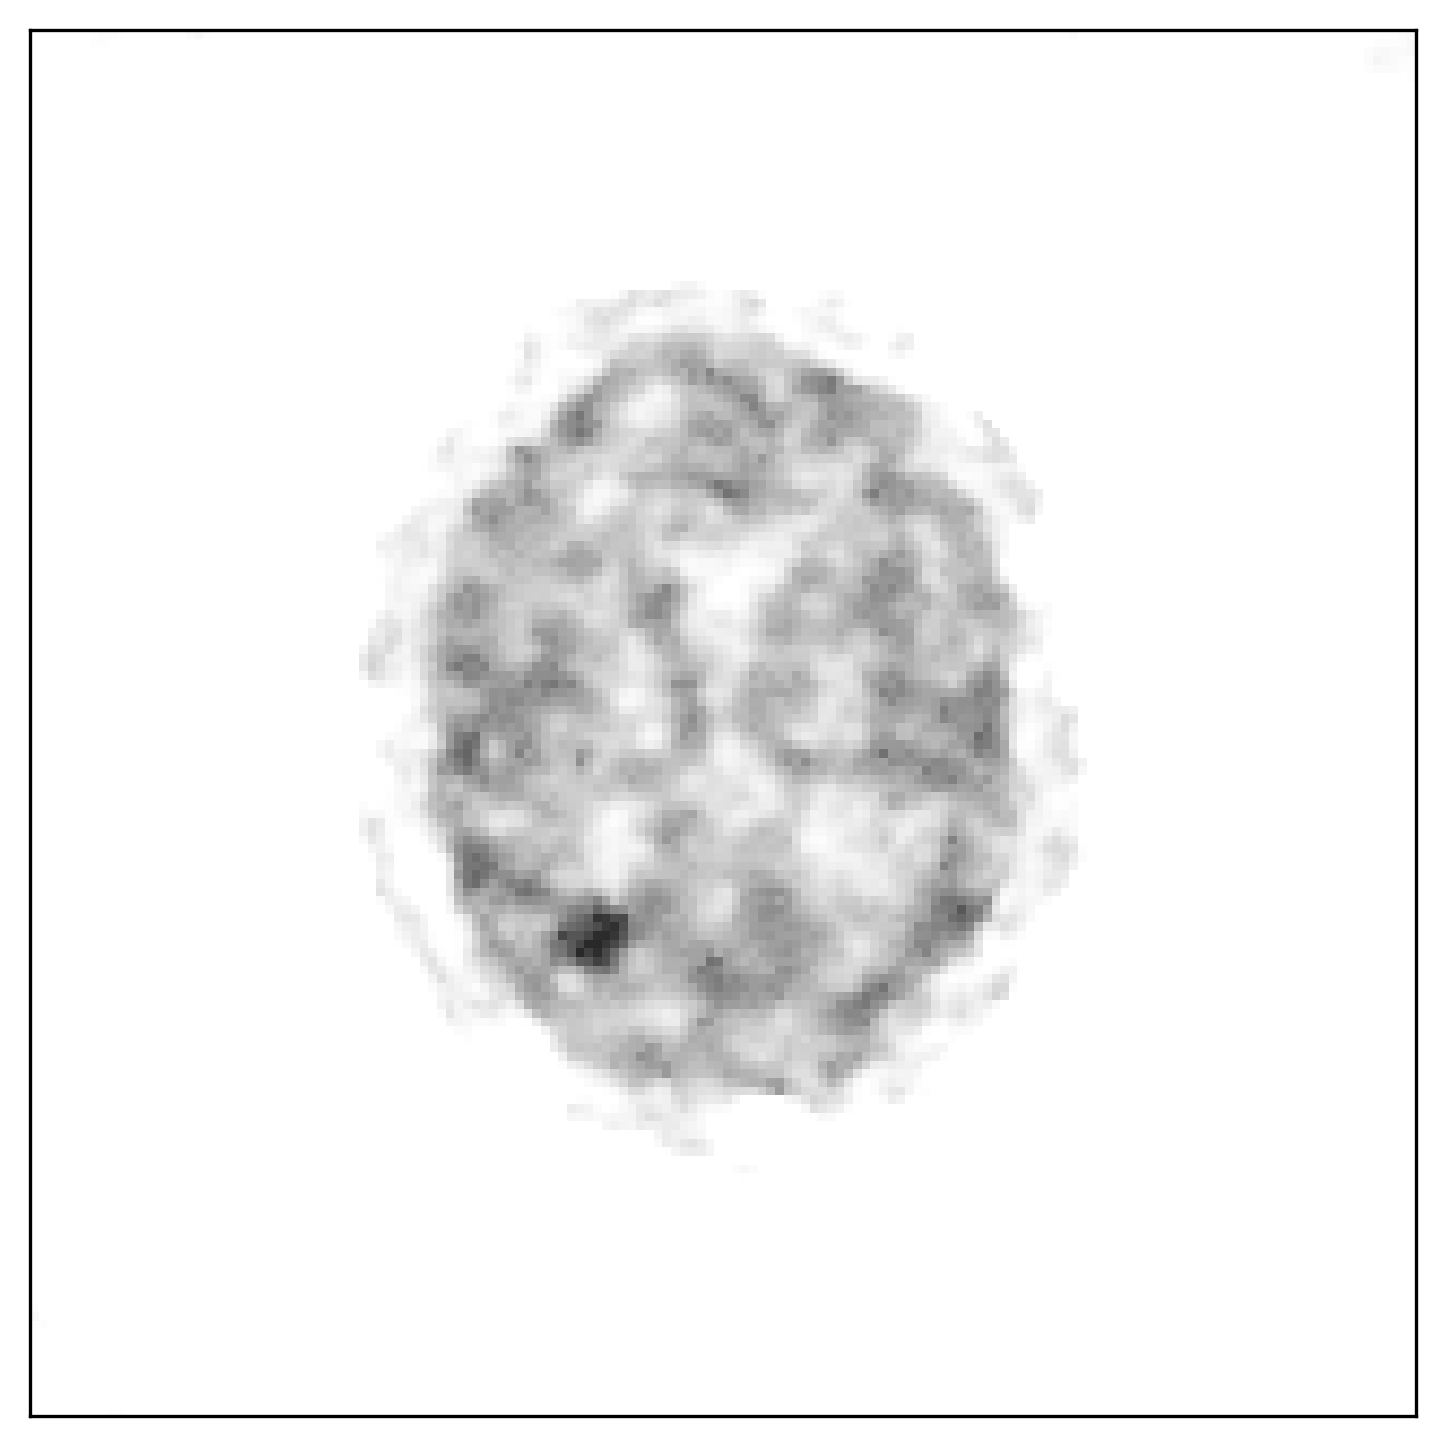
\includegraphics[scale=0.15]{image_to_image/mlem2_denoised.png}};
            \node (recon_full) [right=0.45cm of recon_bin_1, yshift=-1.5cm] {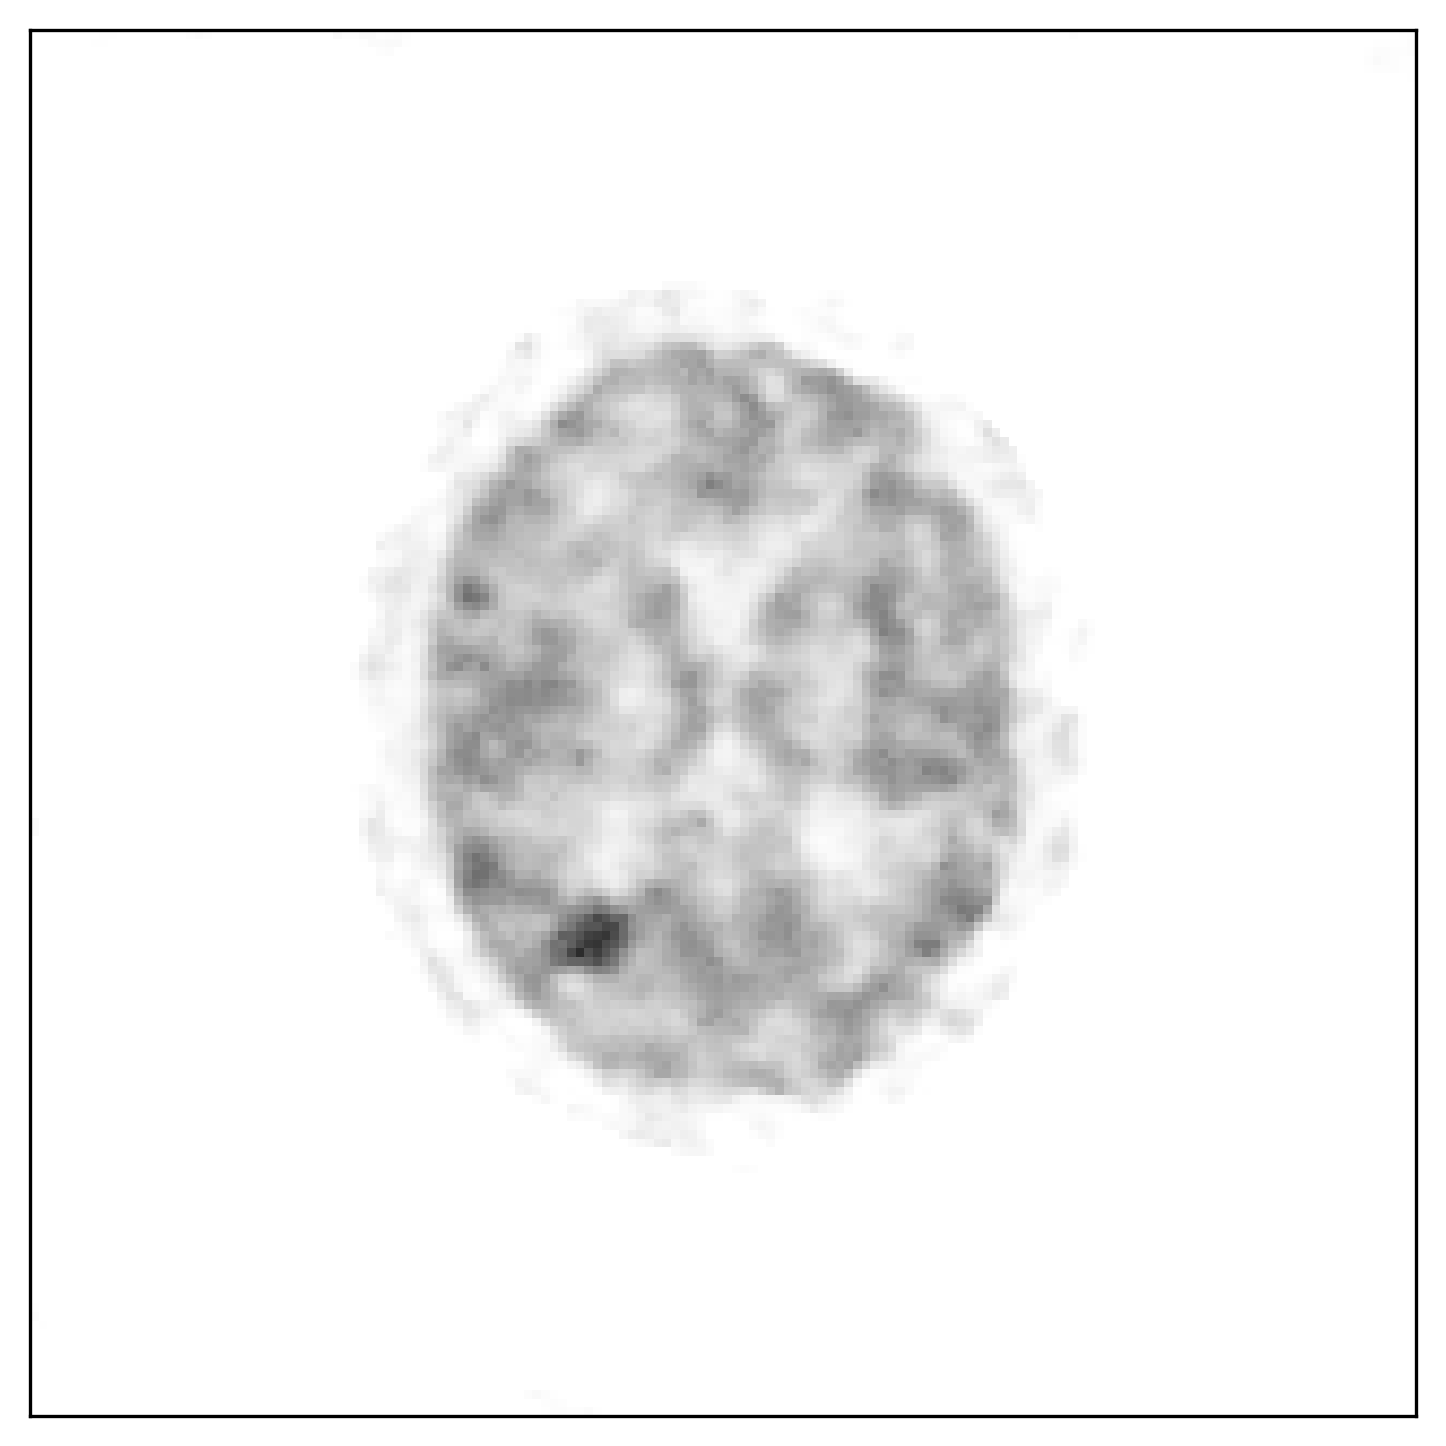
\includegraphics[scale=0.15]{image_to_image/mlem_denoised.png}};

            \draw[->, thick] (full_sino) -- (bin0);
            \draw[->, thick] (full_sino) -- (bin1);
            \draw[->, thick] (bin0) -- (brain_0) node[midway, below] {MLEM};
            \draw[->, thick] (bin1) -- (brain_1) node[midway, above] {MLEM};
            \draw[->, thick] (brain_0) -- (recon_bin_0) node[midway, below] {CNN};
            \draw[->, thick] (brain_1) -- (recon_bin_1) node[midway, above] {CNN};
            \draw[->, thick] (recon_bin_0) -- (recon_full);
            \draw[->, thick] (recon_bin_1) -- (recon_full);

            \draw[<->, thick, orange] (recon_bin_0.north) -- (brain_1.south) node[midway, above, fill=white, inner sep=1pt, yshift=0.15cm] {$\mathcal{L}_{\text{n2n}}$};
            \draw[<->, thick, orange] (recon_bin_1.south) -- (brain_0.north);

        \end{tikzpicture}
    \caption{Noise2Noise training in image domain.}
    \end{figure}
\end{frame}

\begin{frame}{Loss function}{Noise2Noise for PET reconstruction/denoising}
    MSE loss only is biased toward smoothness \cite{Blau2018}
    \begin{figure}
        \centering
        \begin{subfigure}[b]{0.32\textwidth}
            \centering
            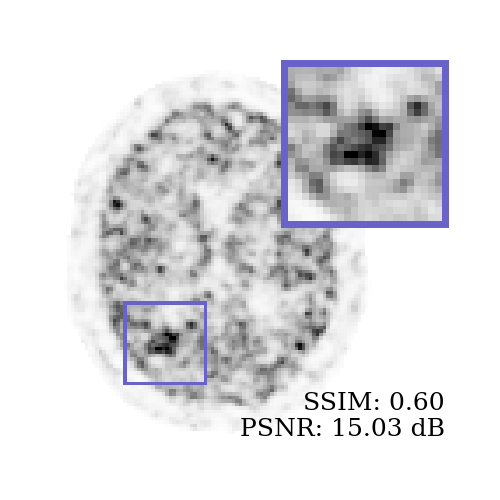
\includegraphics[width=\linewidth]{results/recon_mlem.png}
            \caption{MLEM / noisy sinogram}
            \label{fig:res1}
        \end{subfigure}\hfill
        \begin{subfigure}[b]{0.32\textwidth}
            \centering
            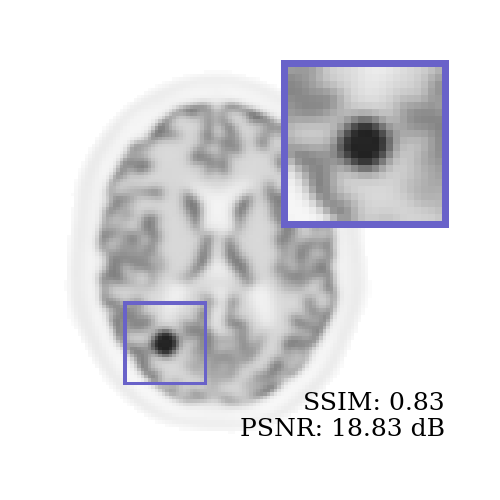
\includegraphics[width=\linewidth]{results/recon_nfpt.png}
            \caption{MLEM / clean sinogram}
            \label{fig:res2}
        \end{subfigure}\hfill
        \begin{subfigure}[b]{0.32\textwidth}
            \centering
            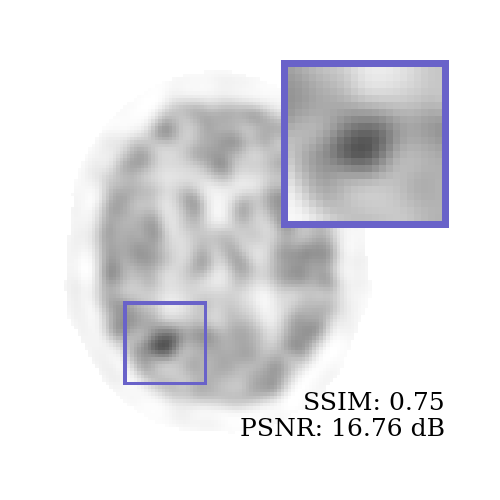
\includegraphics[width=\linewidth]{results/recon_denoised_bias.png}
            \caption{MLEM / denoised by Noise2Noise}
            \label{fig:res3}
        \end{subfigure}
        \caption{Noise2Noise results}
        \label{fig:noise2noise-results}
    \end{figure}
{\color{lightgray}\scriptsize Image source : author}
\end{frame}

\begin{frame}{Loss function}{Noise2Noise for PET reconstruction/denoising}
    \begin{align*}
        \mathcal{L}_{\text{C}}(y^1, y^2, \theta) &= \sum_i \pth{d_{\text{c}}\left(f_\theta(y_i^1), y_i^2\right) + \mu d_{\text{c}}\left(f_\theta(y_i^1), y_i^1\right)},
        \\
        \mathcal{L}_{\text{I}}(y^1, y^2, \theta) &= \sum_i \Bigpth{d\left(f_\theta(\hat{x}_i^1), \hat{x}_i^2\right) + \mu d_{\text{c}}\Bigpth{\fracp{A}{2}f_\theta(\hat{x}_i^1), y_i^1}},
        \\
        \mathcal{L}_{\text{CI}}(y^1, y^2, \theta) &= \sum_i \Bigpth{d_{\text{c}}\Bigpth{\fracp{A}{2}f_\theta(\hat{x}_i^1), y_i^2} + \mu d_{\text{c}}\Bigpth{\fracp{A}{2}f_\theta(\hat{x}_i^1), y_i^1}},
    \end{align*}
    where $\hat{x}(y)$ is an under-regularized solution obtained either with FBP or with the MLEM algorithm, and $d$ and $d_{\text{c}}$ are respectively the L1/L2 loss and a distance measure in the sinogram domain (such as KL).
\end{frame}

\begin{frame}{Results}{Noise2Noise for PET reconstruction/denoising}
    \begin{figure}
    \centering
    \tiny
    % trim : left bottom right top 
    \begin{minipage}{0.07\linewidth}
        \centering
        \vspace{-10pt}
        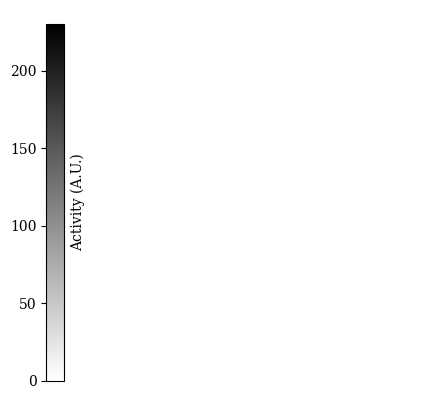
\includegraphics[trim={10 0 358 0},clip, height=80pt]{results_mic/cbar.png}
    \end{minipage}
    \begin{minipage}{0.12\linewidth}
        \centering
        \vspace{5pt}
        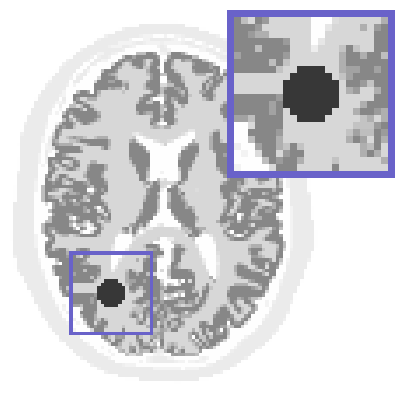
\includegraphics[width=\linewidth,trim={0 20 0 0},clip]{results_mic/gth.png}
        
        Ground truth
    \end{minipage}
    \begin{minipage}{0.79\linewidth}
        \centering
        \begin{tabular}{ccccc}
            \includegraphics[width=0.145\linewidth,trim={45 45 35 40},clip]{results_mic/prompt_fbp.png} &
            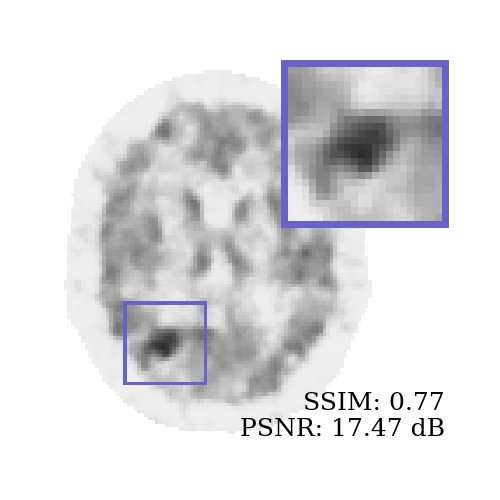
\includegraphics[width=0.145\linewidth,trim={45 45 35 40},clip]{results_mic/image-image_fbp_supervised.png} &
            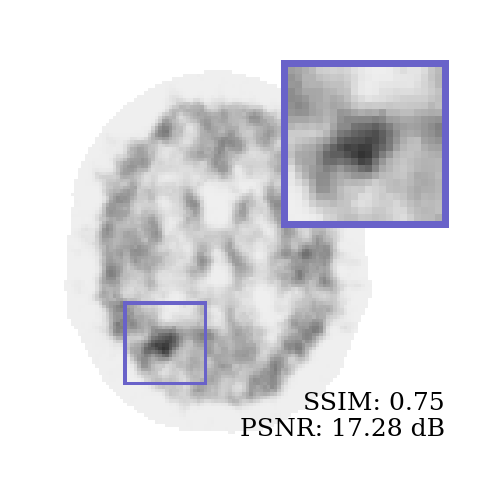
\includegraphics[width=0.145\linewidth,trim={45 45 35 40},clip]{results_mic/image-image_fbp.png} &
            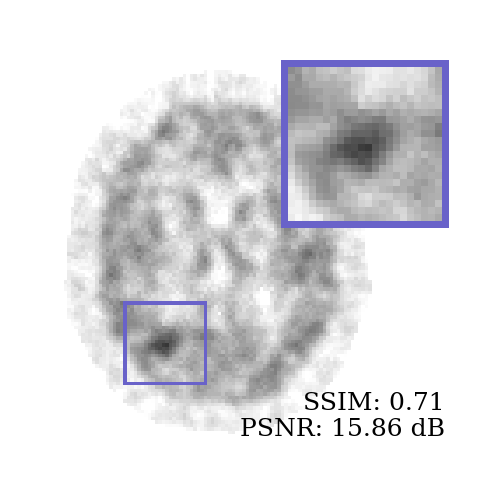
\includegraphics[width=0.145\linewidth,trim={45 45 35 40},clip]{results_mic/photon-photon_fbp.png} &
            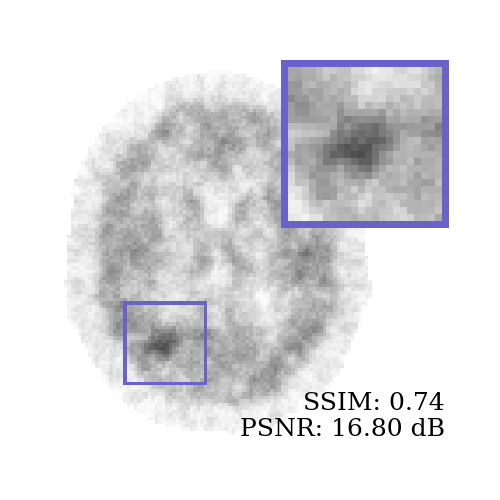
\includegraphics[width=0.145\linewidth,trim={45 45 35 40},clip]{results_mic/photon-image_fbp.png} \\
            Original FBP & $\mathcal{L}^\text{sym}_\text{I}$ (sup) & $\mathcal{L}^\text{sym}_\text{I}$ & $\mathcal{L}^\text{sym}_\text{C}$ & $\mathcal{L}^\text{sym}_\text{CI}$ \\
            & & & & \\
            \includegraphics[width=0.145\linewidth,trim={45 45 35 40},clip]{results_mic/prompt_mlem.png} &
            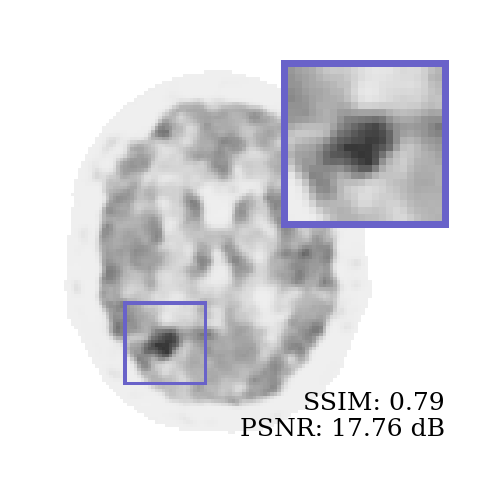
\includegraphics[width=0.145\linewidth,trim={45 45 35 40},clip]{results_mic/image-image_mlem_supervised.png} &
            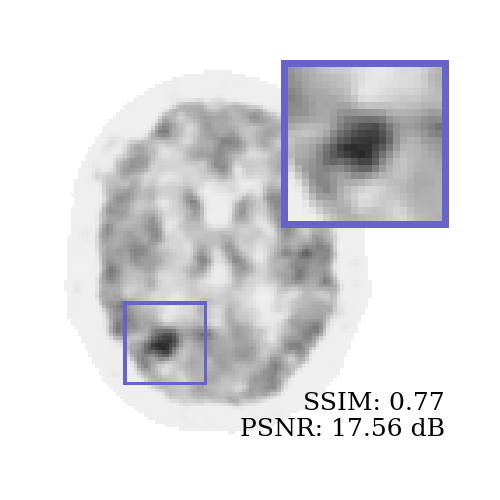
\includegraphics[width=0.145\linewidth,trim={45 45 35 40},clip]{results_mic/image-image_mlem.png} &
            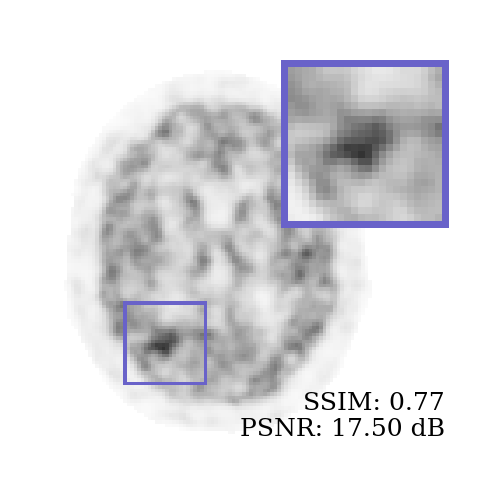
\includegraphics[width=0.145\linewidth,trim={45 45 35 40},clip]{results_mic/photon-photon_mlem.png} &
            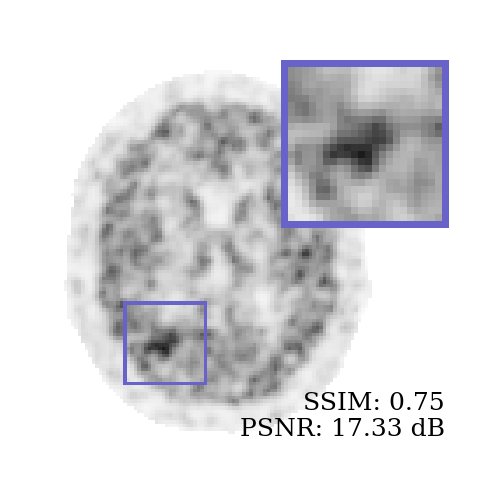
\includegraphics[width=0.145\linewidth,trim={45 45 35 40},clip]{results_mic/photon-image_mlem.png} \\
            Original MLEM & $\mathcal{L}^\text{sym}_\text{I}$ (sup) & $\mathcal{L}^\text{sym}_\text{I}$ & $\mathcal{L}^\text{sym}_\text{C}$ & $\mathcal{L}^\text{sym}_\text{CI}$
        \end{tabular}
    \end{minipage}
    \caption{Results on the BrainWeb phantom. Images are displayed on the same scale.}
    \label{results}
    \end{figure}
\end{frame}

\begin{frame}{Results}{Noise2Noise for PET reconstruction/denoising}
    \begin{figure}
        \centering
        \begin{subfigure}[b]{0.32\textwidth}
            \centering
            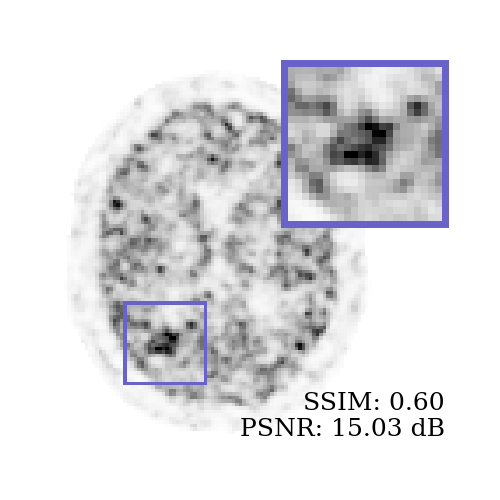
\includegraphics[width=\linewidth]{results/recon_mlem.png}
            \caption{MLEM / noisy sinogram}
            \label{fig:res1}
        \end{subfigure}\hfill
        \begin{subfigure}[b]{0.32\textwidth}
            \centering
            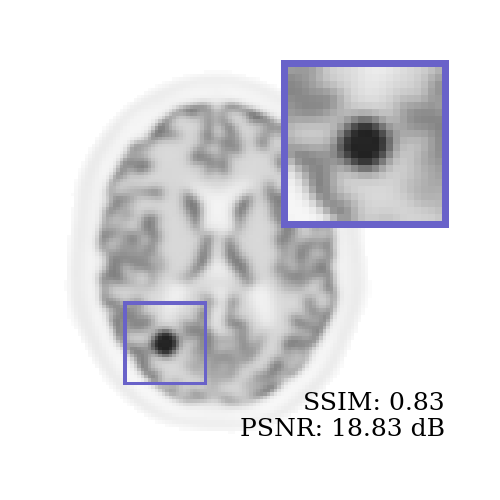
\includegraphics[width=\linewidth]{results/recon_nfpt.png}
            \caption{MLEM / clean sinogram}
            \label{fig:res2}
        \end{subfigure}\hfill
        \begin{subfigure}[b]{0.32\textwidth}
            \centering
            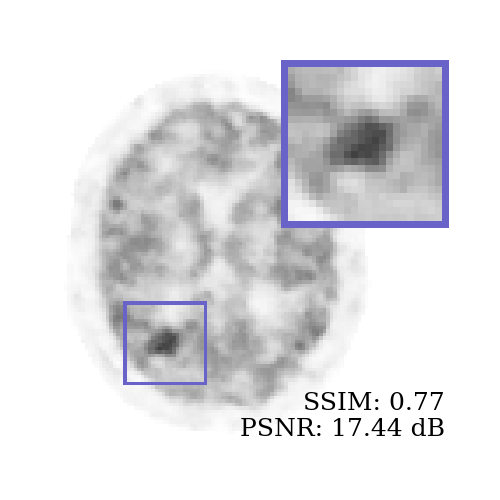
\includegraphics[width=\linewidth]{results/recon_denoised.png}
            \caption{MLEM / denoised by Noise2Noise}
            \label{fig:res3}
        \end{subfigure}
        \caption{Noise2Noise results with data consistency ($\mathcal{L}\CI$) and Gradient Step Denoiser \cite{hureault2021}}
        \label{fig:noise2noise-results_data_consistency}
    \end{figure}
{\color{lightgray}\scriptsize Image source : author}
\end{frame}

\section{Conclusion and Perspectives}

\begin{frame}
    \tableofcontents[currentsection, hideallsubsections]
\end{frame}

\begin{frame}{Conclusion and Perspectives}
    \begin{itemize}
        \item What we have done :
        \begin{itemize}
            \item We have learned a prior from noisy data only, without any clean reference.
            \item We have applied this method to PET image denoising.
            \item This method suits well to PET as Poisson data is $n$-divisible and the statistical conditions are satisfied.
        \end{itemize}
        \item Perspectives :
        \begin{itemize}
            \item Plug-And-Play : Plug learned prior into iterative reconstruction algorithms.
            \item End-to-End : train unrolling networks with Noise2Noise loss.
            \item Train with real PET data from C.H.U de Nantes.
        \end{itemize}
    \end{itemize}
\end{frame}

\begin{frame}{References}
    \tiny
    \printbibliography
\end{frame}

\end{document}